% for sublime text 3
%!TEX root = diss.tex

\chapter{Graph-based Coherence Patterns}
\label{ch:coh-patterns}

In this chapter, we motivate and devise a method for extracting coherence patterns.  
We first provide motivations for representing texts by graphs and for a need of graph-based patterns for coherence modeling (Section \ref{sec:motivation}).  
We then present an algorithm for coherence pattern extraction based on subgraph mining algorithms in graph theory (Section \ref{sec:pattern-extraction}).  
We finally show how extracted coherence patterns can be used to represent the coherence of a text (Section \ref{sec:coh-modeling}) and evaluate coherence patterns and the coherence model on assessing the readability of texts and on generating coherent summaries (Section \ref{sec:exp}). 
We conclude with a summary of main contributions presented in this chapter (Section \ref{sec:summary}). 

\section{Why Graph-based Patterns?}
\label{sec:motivation}

In Chapter \ref{ch:coherence}, we introduced the formal definition of the coherence modeling problem as it is investigated in the research presented in this dissertation. 
We used the ``set'' notation, which is a collection of unordered elements, from mathematics to provide a general formulation.  
We first defined the relation set as a set whose members indicate which sentences in a text are connected to each other. 
Then the concept of coherence pattern is explained as a subset of the relation set (see Definition \ref{def:def-coh-pattern} in Chapter \ref{ch:coherence}). 
Our definitions do not make any assumption about the structure of connections among sentences, in order to give coherence models some flexibility to define or learn such structures. 

In Chapter \ref{ch:rel-work}, we discuss the entity grid 
\cite{barzilay05a,barzilay08} and the entity graph 
\cite{guinaudeau13} coherence models. 
The entity grid model represents the relation set in our definition via a matrix. 
This model makes the definition of coherence patterns more specific by considering sequences, instead of sets, of grammatical transitions.  
It predefines coherence patterns by all possible grammatical transitions of entities across two adjacent sentences. 
The entity graph model employs graphs to represent the relation set of a text.  
It does not extract any pattern, but it makes a strong assumption about the set of all relations among sentences in a text: The bigger the relation set among sentences is, the more coherent the text is. 

However, the entity graph model, without using any pattern, outperforms the entity grid model in experiments performed by \newcite{guinaudeau13}. 
They argue that the entity graph model achieves higher performance in comparison to the entity grid model because the graph representation captures the distribution of entities across adjacent and non-adjacent sentences. 
Graphs are preferred over grids for coherence modeling for two reasons:

\begin{itemize}

	\item They can model long-distance connections between sentences,

	\item They do not encounter the sparsity problem in text representations. 

\end{itemize}

The graph representation of the distribution of entities in a text is transformed into a \mbox{one-mode} projection graph among sentence nodes. 
The average outdegree of nodes in a projection graph measures the extent to which sentence nodes in the graph are connected to each other. 
\newcite{guinaudeau13} assume that the average outdegree metric of a projection graph quantifies the local coherence of its corresponding text. 
Some research papers challenge this assumption (see Chapter \ref{ch:rel-work}) by employing different graph-based metrics with the goal to capture more information about the connectivity of graphs. 
The average outdegree metric is insufficient to measure the connectivity style of relations among nodes in the graph. 
Therefore, it is not a good predictor of the perceived coherence of a text. 
The results of the experiments in this chapter support this claim as well. 

This weakness of the entity graph model motives us to introduce some graph-based features that capture the connectivity style of nodes, how nodes are connected, in projection graphs. 
Considering the linguistics of coherence (see Chapter \ref{ch:coherence}) we hypothesize that coherent texts reveal similar connectivity patterns in their graph representations which make them distinguishable from graph representations of incoherent texts. 
The results of the experiments in this chapter support this hypothesis (Section \ref{sec:exp}). 

In general, the term ``pattern'' refers to some elements which are repeated or which are potentially repeatable. 
From the machine learning perspective, ``pattern'' refers to regularities in data \cite{bishop06}.     
In graph theory, patterns are subgraphs that occur or can potentially occur in graphs \cite{newmanmark10}. 
Graph-based patterns can be extracted using subgraph mining methods. 
These subgraphs are called motifs in graph theory. 
Inspired by linguistic work by \newcite{danes74a}, in the research of this dissertation we refer to the subgraphs extracted from graph representations of texts as connectivity patterns for graphs and coherence patterns for texts.  


\section{Coherence Pattern Extraction}
\label{sec:pattern-extraction}

In Chapter \ref{ch:coherence}, different linguistic theories to coherence patterns are discussed. 
The primary intuition of coherence patterns in the research in this dissertation is inspired by the theory proposed by \newcite{danes74a}. 
What \newcite{danes74a} proposes is that the generalized structure of coherent texts may be described in terms of underlying patterns of transitions between presented information in texts.  
Following entity-based approaches, we take entities mentioned in a text as the pieces of information that make sentences connected. 
The entity graph representation, introduced in Chapter \ref{ch:rel-work}, is employed to model the distribution of entities across sentences of each text in a corpus.  
Then projection graphs of texts are obtained from their entity graph representations.  
Projection graphs model the structure of sentence relations, which are obtained based on the coreferent mentions, in texts. 
We employ a subgraph mining algorithm to automatically extract all connectivity patterns occurring in projection graphs of texts in a corpus as coherence patterns. 
We show that our patterns are similar to the patterns introduced by \newcite{danes74a}. 

\subsection{Background of Graphs}
\label{sec:back-graphs}

The main goal of the research in this dissertation is to represent texts with graphs and then use the connectivity measures of graphs to quantify coherence. 
In order to explain our graph-based method, we need to define some necessary concepts from graph theory.  
We follow \newcite{newmanmark10} to define these terms. 
We refer to them in the rest of the content of this dissertation.  

\paragraph{Graph.}
A \emph{graph} consists of a set of vertices, which are referred to as nodes, and a set of links, which are called edges. 
Following is a formal definition of a graph. 

\begin{definition}
A graph is a pair of two finite sets $G=( V, E )$ where $V$ is a set of nodes and $E$ is a set of edges whose elements are pairs of nodes. 
\end{definition} 
Figure \ref{fig:graph} shows a graph with four nodes and four edges. 

\begin{figure}[!ht]
	\begin{center}
		\begin{tabular}{cc}
			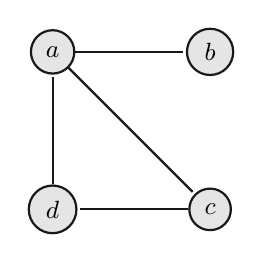
\begin{tikzpicture}[shorten >=1pt,-,scale=0.5]  
				\tikzstyle{node}=[circle,thick,draw=black!90,fill=black!10,minimum size=2mm]
				\tikzstyle{edge}=[draw=black!90, thick]
			   
				 \node [node] (a) at (0,4) {\small{$a$}};
				 \node [node] (b) at (4,4) {\small{$b$}};
				 \node [node] (d) at (0,0) {\small{$d$}}; 
				 \node [node] (c) at (4,0) {\small{$c$}}; 
				 
				 \path[edge] (a) -- (b);
				 %\path[edge] (b) -- (c);
				 \path[edge] (c) -- (d);
				 \path[edge] (d) -- (a);
				 \path[edge] (a) -- (c);
			\end{tikzpicture}
			&
			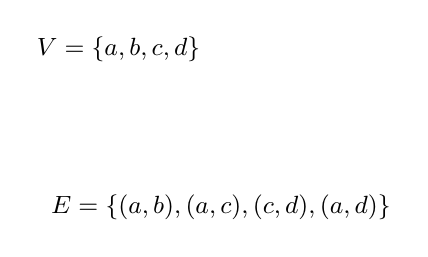
\begin{tikzpicture}[shorten >=1pt,-,scale=0.5]  
				 \node (a) at (0,4) {\small{$V = \left \{ a,b,c,d \right \}$}};
				 \node (b) at (2.6,0) {\small{$E = \left \{(a,b),(a,c),(c,d),(a,d) \right \} $}};
			\end{tikzpicture}
			\\
			$G$ & $V:Nodes$, $E:Edges$ 
		\end{tabular}
	\end{center}
	\caption{$G = (V,E)$ is a graph with node set $V$ and edge set $E$.}
	\label{fig:graph}
\end{figure} 

\paragraph{Directed graphs.}
%
If nodes in a graph are ordered or relations between nodes are not symmetric then pairs in the edge set  of the graph should be interpreted as directed edges. 
A graph whose edges are directed is called a directed graph. 
Figure \ref{fig:dir_graph} shows the directed version of graph $G$ depicted in Figure \ref{fig:graph}, where edge pairs in set $E$ represent directed edges.

\begin{definition}
In a directed graph, an edge $e = (x,y)$ indicates a directed edge from node $x$ towards node $y$, which are called the source node and the target node of edge $e$, respectively. 
\end{definition}

\begin{figure}[!ht]
	\begin{center}
		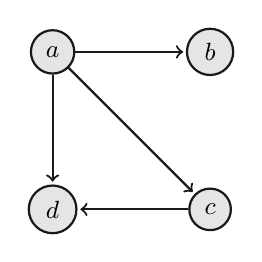
\begin{tikzpicture}[shorten >=1pt, -, scale=0.5]  
			\tikzstyle{node}=[circle,thick,draw=black!90,fill=black!10,minimum size=2mm]
			\tikzstyle{edge}=[draw=black!90, thick]
		   
			 \node [node] (a) at (0,4) {\small{$a$}};
			 \node [node] (b) at (4,4) {\small{$b$}};
			 \node [node] (d) at (0,0) {\small{$d$}}; 
			 \node [node] (c) at (4,0) {\small{$c$}}; 
			 
			 \path[edge,->] (a) -- (b);
			 \path[edge,->] (c) -- (d);
			 \path[edge,->] (a) -- (d);
			 \path[edge,->] (a) -- (c);	       
		\end{tikzpicture}
	\end{center}
	\caption{The directed representation of graph $G$ in Figure \ref{fig:graph}.}
	\label{fig:dir_graph}
\end{figure} 


\paragraph{Isomorphic.}
Two graphs may have an identical connectivity style but different appearances. 
Such graphs are called isomorphic graphs in graph theory. 
More formally, two graphs are isomorphic, if there is an isomorphism relation between the graphs. 

\begin{definition}
	An isomorphism relation between graphs $G_1$ and $G_2$ is an association between node sets of these graphs:
	\begin{equation}
	f: V \left( G_1 \right) \rightarrow V \left( G_2 \right),
	\end{equation}
	such that any two nodes $u$ and $v$ of $G_1$ are adjacent if and only if $f \left( u \right)$ and $f \left( v \right)$ are adjacent in $G_2$. 
\end{definition}

In other words, two graphs $G_1$ and $G_2$ are isomorphic if they fulfill two conditions: 
(i) a one\--to\--one association exists between nodes of $G_1$ and nodes of $G_2$, 
(ii) two nodes of $G_2$ should be connected if and only if their associated nodes in $G_1$ are connected. 
Figure \ref{fig:isomorphic_graph} illustrates two isomorphic graphs and an isomorphic relation between them.  

\begin{figure}[!ht]
	\begin{center}
		\begin{tabular}{c@{\hskip 2.5cm}c@{\hskip 2.5cm}c}

			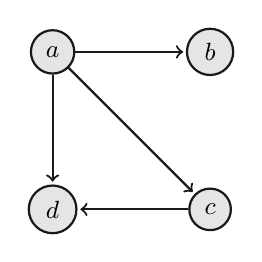
\begin{tikzpicture}[shorten >=1pt,-,scale=0.5]  
				\tikzstyle{node}=[circle,thick,draw=black!90,fill=black!10,minimum size=2mm]
				\tikzstyle{edge}=[draw=black!90, thick]
			   
				 \node [node] (a) at (0,4) {\small{$a$}};
				 \node [node] (b) at (4,4) {\small{$b$}};
				 \node [node] (d) at (0,0) {\small{$d$}}; 
				 \node [node] (c) at (4,0) {\small{$c$}}; 
				 
				 \path[edge,->] (a) -- (b);
				 %\path[edge,->] (b) -- (c);
				 \path[edge,->] (a) -- (c);
				 \path[edge,->] (c) -- (d);
				 \path[edge,->] (a) -- (d);
		       
			\end{tikzpicture}

			 &

		  	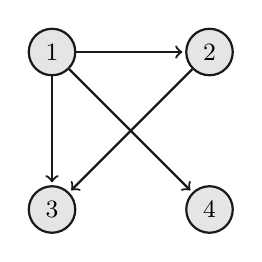
\begin{tikzpicture}[shorten >=1pt,-,scale=0.5]  
			\tikzstyle{node}=[circle,thick,draw=black!90,fill=black!10,minimum size=2mm]
			\tikzstyle{edge}=[draw=black!90, thick]
		   
			 \node [node] (1) at (0,4) {\small{$1$}};
			 \node [node] (2) at (4,4) {\small{$2$}};
			 \node [node] (3) at (4,0) {\small{$4$}}; 
			 \node [node] (4) at (0,0) {\small{$3$}}; 
			 
			 \path[edge,->] (1) -- (2);
			 \path[edge,->] (1) -- (3);
			 \path[edge,->] (1) -- (4);
			 \path[edge,->] (2) -- (4);
		   
		  \end{tikzpicture}

			 &

		  	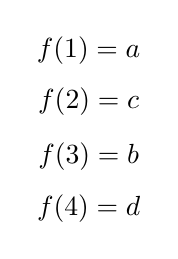
\begin{tikzpicture}[shorten >=1pt,-,scale=0.5]  

			 \node  (1) at (0,4) {$f(1) = a$};
			 \node  (2) at (0,2.7) {$f(2) = c$};
			 \node  (3) at (0,1.3) {$f(3) = b$}; 
			 \node  (4) at (0,0) {$f(4) = d$}; 

		  \end{tikzpicture}
		  \\ $G_1$  &$G_2$ &  $\textit{Node associations}$

		\end{tabular}
	\end{center}
	\caption{Two isomorphic graphs and a sample association between their nodes.}
	\label{fig:isomorphic_graph}
\end{figure} 


\paragraph{Subgraph.} 

Graphs are a pair of two sets: a set of nodes and a set of edges. 
Since each of these sets has several subsets, a graph has several subgraphs as well. 
Following is a formal definition of subgraphs. 

\begin{definition}
	Graph $G_2$ is a subgraph of graph $G_1$ if $G_2$ is isomorphic to a graph whose nodes and edges are subsets of nodes and edges in $G_1$.
\end{definition} 

For example consider graphs $G_1$ and $G_2$ in Figure~\ref{fig:subgraph}. 
Graph $G_2$ is isomorphic with graph $G = \left( \left\{ a,b,c \right\}, \left\{ \left( a , b \right),\left( b , c \right) \right\} \right)$
whose node and edge sets are subsets of the node and edge sets of $G_1$, respectively. 

\begin{figure}[!ht]
	\begin{center}
		\begin{tabular}{c@{\hskip 2.5cm}c@{\hskip 2.5cm}c}
			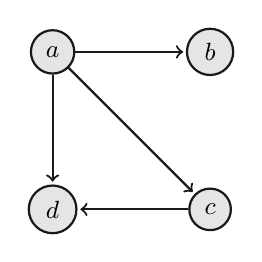
\begin{tikzpicture}[shorten >=1pt,-,scale=0.5]  
				\tikzstyle{node}=[circle,thick,draw=black!90,fill=black!10,minimum size=2mm]
				\tikzstyle{edge}=[draw=black!90, thick]
			   
				 \node [node] (a) at (0,4) {\small{$a$}};
				 \node [node] (b) at (4,4) {\small{$b$}};
				 \node [node] (d) at (0,0) {\small{$d$}}; 
				 \node [node] (c) at (4,0) {\small{$c$}}; 
				 
				 \path[edge,->] (a) -- (b);
				 %\path[edge,->] (b) -- (c);
				 \path[edge,->] (a) -- (c);
				 \path[edge,->] (c) -- (d);
				 \path[edge,->] (a) -- (d);
			\end{tikzpicture}
			&
		  	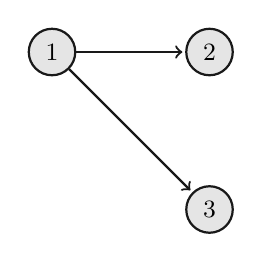
\begin{tikzpicture}[shorten >=1pt,-,scale=0.5]  
				\tikzstyle{node}=[circle,thick,draw=black!90,fill=black!10,minimum size=2mm]
				\tikzstyle{edge}=[draw=black!90, thick]
			   
				 \node [node] (1) at (0,4) {\small{$1$}};
				 \node [node] (2) at (4,4) {\small{$2$}};
				 \node [node] (3) at (4,0) {\small{$3$}}; 
				 
				 \path[edge,->] (1) -- (2);
				 \path[edge,->] (1) -- (3);
		  	\end{tikzpicture}
		  	&
  			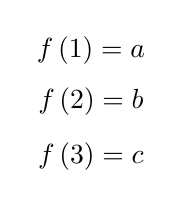
\begin{tikzpicture}[shorten >=1pt,-,scale=0.5]  
				\node  (1) at (0,4) {$f \left( 1 \right) = a$};
	 			\node  (2) at (0,2.7) {$f \left( 2 \right) = b$};
				\node  (3) at (0,1.3) {$f \left( 3 \right) = c$};
			\end{tikzpicture}
			\\
			$G_1$ & $G_2$  & $\textit{Node associations}$

		\end{tabular}
	\end{center}
	\caption{Graph $G_2$ is a subgraph of graph $G_1$.}
	\label{fig:subgraph}
\end{figure} 


\paragraph{K-node (sub)graph.}
The size of a (sub)graph is equal to the size of its node set. 
In Figure \ref{fig:subgraph}, graph $G_2$ is a 3-node subgraph of graph $G_1$. 

\begin{definition}
Graph $G_2 = \left( V_2 , E_2 \right)$ is a k-node subgraph of graph $G_1 = \left( V_1, E_1 \right)$ if $G_2$ is a subgraph of $G_1$, and $V_2$ has $k$ elements, $|V_2|=k$. 
\end{definition}

\paragraph{Induced subgraph.} 
An induced subgraph of a graph is a subgraph of the graph with an extra condition on its edges.  
Edges must connect any two subgraph nodes whose associated nodes in the main graph are connected. 

\begin{definition} 
Graph $G_2 = (V_2, E_2)$ is an induced subgraph of graph $G_1 = (V_1, E_1)$ if $V_2 \subseteq V_1$ and 
$E_2 = \left\{ (x,y)| x \in V_2, y \in V_2, (f(x),f(y)) \in E_1  \right\}$.
\end{definition}

Figure \ref{fig:induced_subgraphs} shows graph $G_1$ and two of its subgraphs $G_2$ and $G_3$.  
Graph $G_2$ is not an induced subgraph of graph $G_1$ because there is no edge between node $1$ and node $3$ in $G_2$ while their associated nodes, $a$ and $b$, in graph $G_1$ are connected. 
In contrast, graph $G_3$ is an induced subgraph of $G_1$ because it contains all possible edges that exist in graph $G_1$. 

\begin{figure}[!ht]
	\begin{center}
		\begin{tabular}{c@{\hskip 1.5cm}c@{\hskip 1.5cm}c@{\hskip 1.5cm}c}
			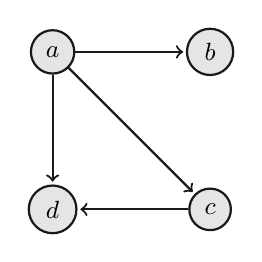
\begin{tikzpicture}[shorten >=1pt,-,scale=0.5]  
				
				\tikzstyle{node}=[circle,thick,draw=black!90,fill=black!10,minimum size=2mm]
				\tikzstyle{edge}=[draw=black!90, thick]
			   
				\node [node] (a) at (0,4) {\small{$a$}};
				\node [node] (b) at (4,4) {\small{$b$}};
				\node [node] (d) at (0,0) {\small{$d$}}; 
				\node [node] (c) at (4,0) {\small{$c$}}; 
				 
				\path[edge,->] (a) -- (b);
				\path[edge,->] (a) -- (c);
				\path[edge,->] (c) -- (d);
				\path[edge,->] (a) -- (d);

			\end{tikzpicture}
	 		&
  			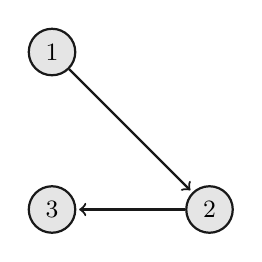
\begin{tikzpicture}[shorten >=1pt,-,scale=0.5]  
	
				\tikzstyle{node}=[circle,thick,draw=black!90,fill=black!10,minimum size=2mm]
				\tikzstyle{edge}=[draw=black!90, thick]
   
	 			\node [node] (1) at (0,4) {\small{$1$}};
	 			\node [node] (2) at (4,0) {\small{$2$}};
	 			\node [node] (3) at (0,0) {\small{$3$}}; 
	 
	 			\path[edge,->] (1) -- (2);
	 			\path[edge,->] (2) -- (3);
  			\end{tikzpicture}
	 		&
  			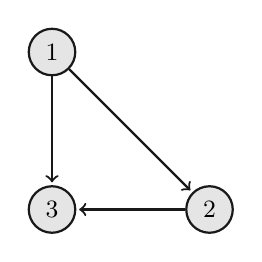
\begin{tikzpicture}[shorten >=1pt,-,scale=0.5]  
	
				\tikzstyle{node}=[circle,thick,draw=black!90,fill=black!10,minimum size=2mm]
				\tikzstyle{edge}=[draw=black!90, thick]
   
				\node [node] (1) at (0,4) {\small{$1$}};
	 			\node [node] (2) at (4,0) {\small{$2$}};
	 			\node [node] (3) at (0,0) {\small{$3$}}; 
	 
	 			\path[edge,->] (1) -- (2);
	 			\path[edge,->] (2) -- (3);
	 			\path[edge,->] (1) -- (3);

  			\end{tikzpicture}
  			&
  			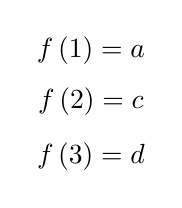
\begin{tikzpicture}[shorten >=1pt,-,scale=0.5]  
	 			\node  (1) at (0,4)   {$f \left( 1 \right) = a$};
	 			\node  (2) at (0,2.7) {$f \left( 2 \right) = c$};
	 			\node  (3) at (0,1.3) {$f \left( 3 \right) = d$}; 
  			\end{tikzpicture}
			\\
			$G_1$ & $G_2$ & $G_3$ & $\textit{Node associations}$

		\end{tabular}
	\end{center}
	\caption{Both graph $G_2$ and $G_3$ are subgraphs of graph $G_1$. In contrast to $G_2$, graph $G_3$ is an induced subgraph of $G_1$.} 
	\label{fig:induced_subgraphs}
\end{figure} 

It is worth mentioning that in this dissertation we mean induced subgraphs when we use the term ``subgraph''.  
However, in cases that the context is not clear we explicitly distinguish them. 

\paragraph{Graph signature.}
%
Given a list of graphs $ \zeta  = \left[ G_1, G_2, \cdots , G_m \right]$, which are called basis graphs, a graph signature of graph $G$ with respect to $\zeta$ is a vector of normalized frequencies of graphs in $\zeta$ in graph $G$:

\begin{equation}
	\phi \left( G \right) = \left( f_1, f_2, f_3, \cdots, f_m \right),
\end{equation}
where  $\phi \left( G \right)$ denotes the graph signature and $f_i$ is the frequency of graph $G_i$ in graph $G$. 
The frequency of graph $G_i$ in graph $G$ is computed as follows:

\begin{equation}
 f_i = \frac{count(G_i, G)}{\sum_{G_j \in \zeta}{count(G_j, G)}}
\end{equation}
where $count(G_i, G)$ is a function which counts the number of occurrences of $G_i$ in graph $G$. 
The reason of using normalized frequency instead of raw count is that normalized frequency cannot become biased to the number of nodes and edges in graph $G$. 
Normalized frequency of a subgraph can also be interpreted as the probability of the subgraph given graph $G$.  

\subsection{Coherence Pattern Mining}

The entity graph representation of a text encodes the distribution of entities across sentences in a text. 
One-mode projection graphs model the connectivity between sentence nodes considering the entities shared by sentences. 
The main contribution of the research in this chapter is to introduce a set of graph-based patterns that encode the structure of connections (i.e.\ the connectivity style) in projection graphs.  
We use the frequencies of different subgraphs occurring in projection graphs to encode the connectivity style of projection graphs and ideally the coherence of texts. 

Given a corpus of texts, we model connections among sentences in each text by its simple projection graph representation, i.e., $P_U$. 
Two sentence nodes are connected in such a projection graph if they share at least one entity node (see Chapter~\ref{ch:rel-work} for more details).  
It leads us to a set of graphs, each of which represents connections among sentences in a text in the corpus.   
We refer to this set as the \emph{graph set}. 

The connectivity of each graph in a graph set can be represented with its graph signature.
The graph signature encodes the connectivity style of a graph into a vector. 
However, for representing the connectivity style of a graph with a graph signature, a list of basis graphs are required (see Section~\ref{sec:back-graphs}).  
We apply a subgraph mining algorithm to projection graphs in the graph set in order obtain all basis graphs for computing graph signatures. 
These basis graphs, which are subgraphs of projection graphs, can be taken as patterns, each of which may have several occurrences in each projection graph. 
That is the why that we refer to these basis graphs and their frequencies as coherence patterns and features, respectively.  
Figure \ref{fig:pattern-extraction} illustrates our approach for extracting coherence patterns.

\begin{figure}[!ht]
	\begin{center}
		\begin{tikzpicture}
			\node[] (dataset1) at (0,10)  {\includegraphics[scale=0.20] {../figures/text.jpeg}};
			\node[] (eg1) 	   at (0,6)   {\includegraphics[scale=0.05] {../figures/bg1.png}};
			\node[] (proj1)    at (0,2.2) {\includegraphics[scale=0.05] {../figures/proj1.png}};

			\path[->, thick] (dataset1) edge  (eg1);
			\path[->, thick] (eg1) edge  (proj1);



			\node[] (dataset2) at (3,10)  {\includegraphics[scale=0.20]{../figures/text.jpeg}};
			\node[] (eg2) 	   at (3,6)   {\includegraphics[scale=0.05]{../figures/bg1.png}};
			\node[] (proj2)    at (3,2.2) {\includegraphics[scale=0.05]{../figures/proj1.png}};
			\path[->, thick] (dataset2) edge  (eg2);
			\path[->, thick] (eg2) edge  (proj2);



			\node[] (eg) at (6,8) {...};

			\node[] (dataset3) at (9,10)  {\includegraphics[scale=0.20]{../figures/text.jpeg}};
			\node[] (eg3) 	   at (9,6)	  {\includegraphics[scale=0.05]{../figures/bg1.png}};
			\node[] (proj3)    at (9,2.2) {\includegraphics[scale=0.05]{../figures/proj1.png}};
			\path[->, thick] (dataset3) edge  (eg3);
			\path[->, thick] (eg3) edge  (proj3);
			
			
			\node[] (minesg) at (5,-2.2) {\includegraphics[scale=0.5]{../figures/3node.jpg}};
			\path[->, thick] (proj1) edge (minesg);
			\path[->, thick] (proj2) edge (minesg);
			\path[->, thick] (proj3) edge (minesg);
			
		\end{tikzpicture}
	\end{center}
	\caption{An illustration of the approach employed for extracting coherence patterns.}
	\label{fig:pattern-extraction}
\end{figure}


\paragraph{The gSpan Method.}
%
Coherence patterns are subgraphs that occur at least once in one of the projection graphs of texts in a corpus. 
Mining all subgraphs that occur in graphs of a graph set is computationally expensive and is proved to be an NP-complete problem \cite{althaus04}. 
Intuitively, a graph with $|E|$ edges, potentially has $\mathcal{O} \left( 2^{| E |} \right)$ subgraphs.  
A graph with $| V |$ nodes at most has  $\frac{(| V |-1)(| V |-2)}{2}$ edges which is in order of $\mathcal{O} \left( | V | ^2 \right)$. 
So the number of subgraphs in a graph is an exponential order of the squared number of nodes in the graph. 

The goal of the research in this thesis is not to develop an algorithm for mining subgraphs.  
This problem has been extensively studied in computer science, and different algorithms and packages have also been developed for it. 
The gSpan algorithm \cite{yanxifeng02} is one of the efficient methods for mining subgraphs from graphs in a graph set. 
Here, we briefly describe the idea and the method of the gSpan algorithm.  
Interested readers may find more information about the exact algorithm of gSpan in \newcite{yanxifeng02}. 

The gSpan, which stands for \underline{g}raph-based \underline{S}ubstructure \underline{pa}tter\underline{n} mining, algorithm is an approach for extracting all connectivity patterns (i.e.\ subgraphs) that occur in graphs of a graph set. 
It discovers all subgraphs without generating the candidates, so
it is efficient in terms of computation time and memory usage. 
The gSpan method orders graphs in a graph set with respect to their structures.
It then adapts a Depth-First-Search (DFS)  strategy to extract connected subgraphs efficiently. 
It begins with subgraphs with only two nodes and expands them to larger subgraphs. 
We use gSpan to extract patterns from projection graphs. 
These patterns are basis graphs for graph signatures in our model.  

\section{Coherence Modeling}
\label{sec:coh-modeling}

Here, we explain how patterns, which are extracted by gSpan, can be used to measure the coherence of a text. 
Given a corpus of texts, we employ the entity graph to represent the entity distribution across sentences of each text in the corpus. 
We apply a one-mode projection on each entity graph to construct a projection graph (i.e.\ $P_U$) over the sentence nodes of the entity graph. 
The projection graph models the overall entity-based relationships among sentences. 

The output of the subgraphs mining method consists of subgraphs in different sizes.   
Involving subgraphs with different sizes for computing graph signatures results in subgraphs whose frequencies might be dependent on one another. 
Moreover, small subgraphs are likely to occur inside large subgraphs. 
This type of features is advised to be supplied separately to machine learning methods \cite{aggarwalcharu18}. 
So, we extract all possible k-node subgraphs (i.e.\ coherence patterns) which occur in projection graph representations of texts in the corpus. 
The parameter k controls the size of subgraphs.  
Controlling the size of subgraphs helps to run the subgraph mining algorithm more efficiently in terms of the computational time.
Besides, it controls the number of possible subgraphs that can be extracted: large values of k yield many possible graphs with the size of k. 

Assume that $m$ coherence patterns, i.e.\ k-node subgraphs, are mined from all graph representations of texts in a corpus, the coherence of a text is encoded by a vector of frequencies of these patterns in the graph representation of the text. 
More formally, the coherence of  text $d$ is represented by a vector as follows: 

\begin{equation}
Coh(T) \approx <f_0,f_1,f_2,...,f_m>
\end{equation}
where $f_i$ represents the frequency of the $i${th} pattern in the graph representation of text $T$. 

This vector representation of coherence is identical with the graph signature concept in graph theory (see Section \ref{sec:back-graphs}). 
As these vectors can be used to model the similarities and dissimilarities in connectivity structures of graphs, they can also model similarities and dissimilarities of connectivity structures of sentences in a text, which matches our definition of coherence vector in Chapter \ref{ch:coherence}.   
From the machine learning viewpoint, these vectors can be viewed as feature vector representations of coherence. 
Each element of a vector is a feature which represents one aspect of the connectivity structure of sentences in a text. 
Consequently, these feature vectors can be supplied to a machine learning model in order to rank texts with respect to their coherence. 
A machine learning model during training learns to map a feature vector to a score, which can be interpreted as a coherence score, such that the score of a more coherent text be higher than the score of a less coherent one. 
More formally, given two texts $d$ and $d^\prime$ if text $d$ is more coherent than text $d^\prime$ then a machine learning model learns parametric function $\beta$ such that 

\begin{equation}
\beta (d_v) > \beta (d^\prime_v),
\end{equation}
where $d_v$ and $d^\prime_v$ are the feature vectors representing the coherence property of these texts. 

\section{Experiments}
\label{sec:exp}

In this section, we perform a set of experiments to assess coherence patterns and features discussed in this chapter. 
We first investigate how patterns and their frequencies behave on encoding coherence in comparison to the average outdegree.  
We then examine how the size of patterns affects the predictive power of our features for distinguishing graph representations of coherent texts against incoherent ones. 

To this end, we limit the size of patterns by fixing parameter k in the model, which equals to the number of nodes in subgraphs (see Section \ref{sec:coh-modeling}), resulting in two sets of patterns. 
One set consists of subgraphs with three nodes, 3-node patterns, and the other set contains subgraphs with four nodes, which are referred to as 4-node patterns.  
There are no criteria on the number of edges in subgraphs.  

We begin with extracting 3-node subgraphs in order to examine the soundness of mined coherence patterns.  
3-node subgraphs are the smallest meaningful patterns that can model the connectivity style of sentence nodes in projection graphs. 
There is only one 2-node subgraph, $G = \left( V = \lbrace a,b \rbrace, E=\lbrace \left( a, b \right) \rbrace \right)$, whose frequency in any projection graph is equal to the number of edges in the graph. 
Its interpretation is identical with the interpretation of the average outdegree applied by the entity graph model.  
3-node subgraphs are too small and therefore are very likely to occur in most projection graphs in a graph set. 
Moreover, in order to analyze impacts of the size of patterns, we extract 4-node subgraphs to have more informative representations of the connectivity style of graphs. 

As we discussed in Chapter \ref{ch:coherence}, coherence is better to be evaluated in an extrinsic fashion. 
It is mainly because annotating texts for coherence is quite expensive and controlling all conditions for annotators is very difficult \cite{karamanis04a}. 
In the research in this thesis, we focus on two extrinsic evaluation tasks: readability assessment and automatic text summarization. 
The former one is used to evaluate the predictive power of different proposed coherence features by computing the correlation between the values of the coherence features and the readability ratings assigned by human judges. 
We also check how well coherence features can rank texts with respect to their readability levels. 
The summarization task is a specific instance of text generation, where a subset of informative sentences in a text should be extracted and presented in a proper order to generate a coherent and readable summary. 
In this experiment, we evaluate the capabilities of our coherence patterns in producing coherent summaries. 
We show that by integrating our coherence patterns into a graph-based text summarizer \cite{parveen15a}, the performance of the summarizer improves in terms of ROUGE metrics and human qualitative evaluations.

\subsection{Readability Assessment}
\label{sec:readability_assessment}

Readability assessment is about how well a text is understandable for its readers.  
Possible applications of readability assessment are automatic text summarization and simplification systems. 
Measuring readability can also be used in question answering and knowledge extraction systems to prune texts with low readability \cite{kate10}. 

Readability assessment is a challenging task since various factors influence the processing time of a text for its readers.
Accordingly, different features related to syntactic and semantic properties of texts have been used to assess readability. 
These features include shallow features \cite{flesch48,kincaid75}, language modeling features \cite{siluo01,collins-thompson04}, syntactic features \cite{schwarm05} and the text flow or coherence \cite{barzilay08,pitler08}. 
In the research of this dissertation, the readability assessment task mainly is utilized to evaluate the impact of features that represent coherence in quantifying the difficulty of texts.  
In a coherent text, each sentence has some connections with other sentences. 
Although these local connections somewhat make texts easy-to-read, none of the entity transition features introduced in the entity grid model \cite{barzilay08} significantly correlate with readability ratings assigned by human judges \cite{pitler08}.  
It is shown that the entity graph representations of the entity distribution across sentences provide more informative representation than the entity grid model (See Chapter \ref{ch:rel-work}).  
Here, we first investigate if the average outdegree metric proposed by the entity graph model strongly correlates with readability ratings. 
We also use this experiment to evaluate and interpret our coherence patterns. 

It is worth to emphasize that the readability of a text is, of course, beyond the coherence of the text. 
That is why we do not use our features to predict the exact readability ratings associated with texts. 
However, since coherence is one of the crucial factors for readability assessment, easy-to-read texts imply to be coherent as well. 
We expect that the values of our features show a considerable correlation with human-provided readability scores associated with texts. 
In another experiment, we also check how well we can rank texts with respect to their readability if only coherence has been taken into account. 


\subsubsection{Data}
\label{sec:data_pitler}

We utilize the dataset collected by \newcite{pitler08}, which consists of thirty articles randomly selected from the Wall Street Journal (WSJ) corpus. 
These articles are intended for an educated adult audience implying that they are well-written and free of grammatical errors. 
The articles were rated by three human judges on a scale from $1$ to $5$, where a higher rating indicates an easier-to-read article. 
Each of the judges had unlimited time to read the articles and assign the ratings. 
Human judges received following questions \cite{pitler08}:

\begin{itemize}
    \item How well-written is the article?
    \item How well does the article fit together?
    \item How easy was it to understand?
    \item How interesting is the article?
\end{itemize} 
 
\newcite{pitler08} state that since in most cases judges gave the same rating to all questions, they only consider the given rates for the first question (``How well-written is the article?''). 
Then the average of ratings for this question is defined as the final rating of a text. 
That is the reason that they also use these scores for coherence evaluations \cite{pitler08}. 
This dataset is suitable for coherence evaluation because its articles appeared in the Wall Street Journal and are aimed at the same target audience. 
Therefore, the quality of articles relates to the discourse features such as coherence rather than surface features. 
The text presented in Example~\ref{ex:wsj-1818} is one\footnote{The ID of the article is WSJ-1818.} of the articles in this dataset with the final human readability score of 3.7 out of five.  


\begin{examples}
	\label{ex:wsj-1818}
	The Associated Press's earthquake coverage drew attention to a phenomenon that deserves some thought by public officials and other policy makers. 
	Private relief agencies, such as the Salvation Army and Red Cross, mobilized almost instantly to help people, while the Washington bureaucracy ``took hours getting into gear.'' 
	One news show we saw yesterday even displayed 25 federal officials meeting around a table. 
	We recall that the mayor of Charleston complained bitterly about the federal bureaucracy's response to Hurricane Hugo. 
	The sense grows that modern public bureaucracies simply don't perform their assigned functions well. 
\end{examples}

We exclude one article from the dataset to make the texts consistent in style; for instance one of these articles is a poem that follows a totally different style from other articles.  
Two articles are not available. 
The final list of articles that are used from this dataset in the experiments presented in this dissertation is as follows:
\emph{
WSJ\_0068,
WSJ\_0177,
WSJ\_0232,
WSJ\_0311,
WSJ\_0402,
WSJ\_0494,
WSJ\_0613,
WSJ\_0663,
WSJ\_0717,
WSJ\_0744,
WSJ\_1011,
WSJ\_1027,
WSJ\_1043,
WSJ\_1281,
WSJ\_1324,
WSJ\_1472,
WSJ\_1520,
WSJ\_1724,
WSJ\_1746,
WSJ\_1773,
WSJ\_1784,
WSJ\_1818,
WSJ\_1906,
WSJ\_2121,
WSJ\_2238,
WSJ\_2336, } and \emph{WSJ\_2339}. 

\subsubsection{Feature Analysis}
The goal of this experiment is to investigate the correlation of different features for representing coherence with readability ratings associated with the articles. 
To this end, we represent each article in the dataset by its entity graph, where entities are obtained heuristically by string matching among all nouns in an article. 
We apply a one-mode projection to obtain projection graphs, more specifically $P_U$. 
This projection graph captures the entity-based connectivity between sentences of articles. 
Given projection graphs of every article in the dataset, we compute the Pearson correlation between the values of a feature and readability ratings associated with articles. 
We use the Pearson correlation because feature values and ratings are meaningful by themselves. 
However, other correlation assessment methods such as the Spearman correlation could also be used to check how well rankings of texts based on these features values correlate with each other. 
However, the Spearman's rank correlation coefficient cannot be used as a significant measure of the strength of the association between variables \cite{hauke11}.
Furthermore, \newcite{pitler08} employ the Pearson correlation coefficient to evaluate entity transition features extracted from the entity grid representation \cite{barzilay08} of texts for the readability assessment task. 
Our experiments, here, follow their research direction, so we also use the Pearson correlation. 

\paragraph{The Pearson correlation coefficient.} 
The Pearson correlation coefficient is a measure of the linear correlation between the values of two variables. 
In our experiments, variables are coherence features and readability ratings, which are assigned to articles by human judges.  
The Pearson correlation coefficient, $\rho$, ranges between $-1$ and $+1$. 
A high absolute value of $\rho$ shows a strong correlation between the input variables. 
The sign of $\rho$ indicates the direction of the relationship between examined variables. 
In extreme cases, $+1$ shows a total positive linear correlation, $0$ is no linear correlation, and $-1$ is a total negative linear correlation. 
The Pearson correlation also measures how statistically significant examined variables are correlated. 
This measure is referred to by p\_value. 
We consider correlations with \mbox{p\_value < 0.05} statistically significant. 
We evaluate the following features: average outdegree, frequencies of 3-node patterns, and frequencies of 4-node patterns. 

\paragraph{Experimental settings.} 
In order to be compatible with the entity grid features that are evaluated by \newcite{pitler08}, we use the gold parse trees in the Penn Treebank II \cite{marcus94} to extract all nouns in an article as mentions. 
All nouns with identical stems are taken to be coreferent to the same entity. 
The Stemmer class from Stanford CoreNLP\footnote{V3.2.0, 2013-06-19} is employed in this regard. 

The subgraph mining and primary subgraph counting parts are performed by the Java implementation of the gSpan algorithm which is also publicly available\footnote{\url{http://www.cs.ucsb.edu/~xyan/software/gSpan.htm}}. 
This package counts all subgraphs, but it does not take care whether a subgraph is induced or not. 
Since we are interested in only induced subgraphs we employ SageMath\footnote{\url{http://sagemath.org/download- linux.html}} for counting induced subgraphs in each graph.  
For computing the Pearson correlation between feature values and readability ratings, we use the implementation of this metric in R\footnote{Version: V3.2.0}. 

\paragraph{Mined Coherence Patterns.} 
Figure \ref{fig:3node-patterns} shows 3-node patterns, which are extracted from projection graph representations of texts in the examined readability dataset. 
There is an order between nodes $s_t < s_u < s_v$, where ``$<$'' is the sign of preceding: Sentence $s_t$ appears before both $s_u$ and $s_v$ in the input text, and sentence $s_u$ precedes $s_v$. 

\begin{figure}[!ht]

	\begin{center}

		\resizebox{\columnwidth}{!}
		{%
			\begin{tabular}{@{}c@{\hskip 1.5cm}c@{\hskip 1.5cm}c@{\hskip 1.5cm}c@{}}
				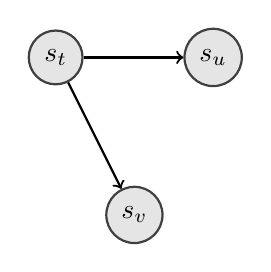
\begin{tikzpicture}  
		        	\tikzstyle{sentence}=[circle,thick,draw=black!75,fill=black!10,minimum size=5mm]
		        	\tikzstyle{edge}=[draw, thick]
		       		\begin{scope}
		         		\node [sentence] (s1) at (0,2) {$s_t$};
				        \node [sentence] (s2) at (2,2) {$s_u$};
				        \node [sentence] (s3) at (1,0) {$s_v$}; 
				        
				        \path[edge,->] (s1) edge  (s2);
				        \path[edge,->] (s1) edge  (s3);
		        	\end{scope}        
		      	\end{tikzpicture}
				&
		 		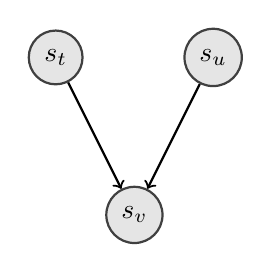
\begin{tikzpicture} 
		        	\tikzstyle{sentence}=[circle,thick,draw=black!75,fill=black!10,minimum size=5mm]
		        	\tikzstyle{edge}=[draw, thick]
		       		\begin{scope}
		         		\node [sentence] (s1) at (0,2) {$s_t$};
		         		\node [sentence] (s2) at (2,2) {$s_u$};
		         		\node [sentence] (s3) at (1,0) {$s_v$}; 
		         
		         		\path[edge,->] (s1) edge  (s3);
		         		\path[edge,->] (s2) edge (s3);
		        	\end{scope}        
		      	\end{tikzpicture}
		      	&

				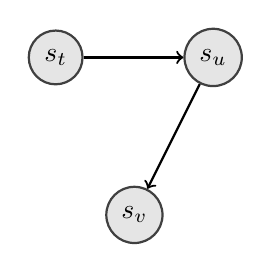
\begin{tikzpicture}
		        	\tikzstyle{sentence}=[circle,thick,draw=black!75,fill=black!10,minimum size=5mm]
		        	\tikzstyle{edge}=[draw, thick]
		       		\begin{scope}
		         		\node [sentence] (s1) at (0,2) {$s_t$};
		         		\node [sentence] (s2) at (2,2) {$s_u$};
		         		\node [sentence] (s3) at (1,0) {$s_v$}; 
		         		
		         		\path[edge,->] (s1) edge (s2);
		         		\path[edge,->] (s2) edge (s3);
		        	\end{scope}        
		      	\end{tikzpicture}
		 		&
		 		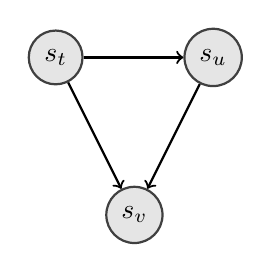
\begin{tikzpicture}  
		        	\tikzstyle{sentence}=[circle,thick,draw=black!75,fill=black!10,minimum size=5mm]
		        	\tikzstyle{edge}=[draw, thick]
		       		\begin{scope}
		        		\node [sentence] (s1) at (0,2) {$s_t$};
		         		\node [sentence] (s2) at (2,2) {$s_u$};
		         		\node [sentence] (s3) at (1,0) {$s_v$};
		         
		         		\path[edge,->] (s1) edge (s2);
		         		\path[edge,->] (s1) edge (s3);
		         		\path[edge,->] (s2) edge (s3);
		        	\end{scope}        
		      	\end{tikzpicture}
		      	\\
		      	$p_1$& $p_2$ & $p_3$ & $p_4$
		\end{tabular}
	}%
	\end{center}
	\caption{Extracted 3-node patterns from the readability dataset. Nodes are in order $s_t<s_u<s_w$ to show the order of sentences in a text.}
	\label{fig:3node-patterns}
\end{figure}

We interpret these patterns as follows:

\begin{itemize}
    \item \boldmath{$p_1$}\textbf{:} 
    A sentence is connected with two of its subsequent sentences.
    More precisely, at least two entities are mentioned in one sentence, i.e.\ $s_t$, and the subsequent ones, i.e.\ $s_u$ and $s_v$,  are about those entities. 
    This pattern is similar to two coherence patterns that are defined by \newcite{danes74a}, i.e.\ pattern 2 and pattern 3 illustrated in Table \ref{tab:danesh_coherence_patterns}. 

    \item \boldmath{$p_2$}\textbf{:} 
    The connection between two sentences is made by a subsequent sentence of those sentences. 
    This patterns indicates that entities in $s_t$ and $s_u$ are connected to each other in $s_v$. 
     

    \item \boldmath{$p_3$}\textbf{:} 
    Each sentence tends to refer to an entity in its immediately preceding sentence. 
    The absence of a connection between $s_t$ and $s_v$ indicates that the entity that connects $s_t$ and $s_u$ is different from the entity that connects $s_u$ and $s_v$. 
    This pattern roughly reminds us of the center shift in the centering theory. 
    This pattern is also similar to the linear pattern proposed by \newcite{danes74a}, i.e.\ pattern 1 depicted in Table \ref{tab:danesh_coherence_patterns}. 

    \item \boldmath{$p_4$}\textbf{:} 
    This pattern encodes three sentences that all are connected with each other. 
    Entities that connect sentences are not necessarily unique. 
    An essential property of this pattern is that it has the maximum number of edges showing many repetitions of entities among sentences. 
\end{itemize}

Figure \ref{fig:4node-patterns} shows all subgraphs with four nodes that are extracted from the projection graphs corresponding to texts in the readability dataset. 
These 4-node subgraphs have more capacity than 3-node subgraphs for capturing connectivity information, because 4-node patterns contain more nodes and therefore more possible edges. 
So they are expected to distinguish texts better than 3-node patters.  

\begin{figure}[!ht]
	\begin{center}
		\resizebox{\columnwidth}{10cm}
		{%
		\begin{tabular}{@{}c@{\hskip 1.5cm}c@{\hskip 1.5cm}c@{\hskip 1.5cm}c@{}}
			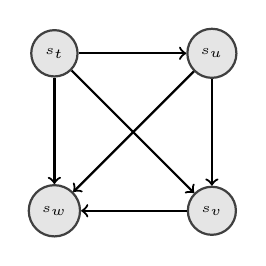
\begin{tikzpicture}
        		\tikzstyle{sentence}=[circle,thick,draw=black!75,fill=black!10,minimum size=1mm]
        		\tikzstyle{edge}=[draw, thick,->]
       			\begin{scope}
			    	\node [sentence] (s1) at (0,2) {\tiny{$s_t$}};
			        \node [sentence] (s2) at (2,2) {\tiny{$s_u$}};
			        \node [sentence] (s3) at (2,0) {\tiny{$s_v$}};
			        \node [sentence] (s4) at (0,0) {\tiny{$s_w$}};  
			        \path[edge] (s1) edge [above] node[font=\tiny] {} (s2);
			        \path[edge] (s1) edge [above] node[font=\tiny] {} (s3);
			        \path[edge] (s1) edge [above] node[font=\tiny] {} (s4);
			        \path[edge] (s2) edge [above] node[font=\tiny] {} (s4);
			        \path[edge] (s2) edge [above] node[font=\tiny] {} (s3);
			    	\path[edge] (s3) edge [above] node[font=\tiny] {} (s4);
		        \end{scope}        
    	    \end{tikzpicture}
			&
			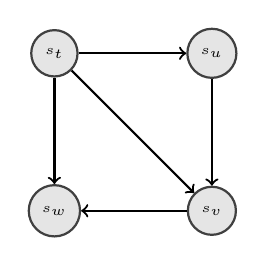
\begin{tikzpicture}
			    \tikzstyle{sentence}=[circle,thick,draw=black!75,fill=black!10,minimum size=2mm]
			    \tikzstyle{edge}=[draw, thick, ->]
			    \begin{scope}
					\node [sentence] (s1) at (0,2) {\tiny{$s_t$}};
			        \node [sentence] (s2) at (2,2) {\tiny{$s_u$}};
			        \node [sentence] (s3) at (2,0) {\tiny{$s_v$}};
			        \node [sentence] (s4) at (0,0) {\tiny{$s_w$}};  
			        \path[edge] (s1) edge [above] node[font=\tiny] {} (s2);
			        \path[edge] (s1) edge [above] node[font=\tiny] {} (s3);
			        \path[edge] (s1) edge [above] node[font=\tiny] {} (s4);
			        \path[edge] (s2) edge [above] node[font=\tiny] {} (s3);
			        \path[edge] (s3) edge [above] node[font=\tiny] {} (s4);
			    \end{scope}        
			\end{tikzpicture}
			&
			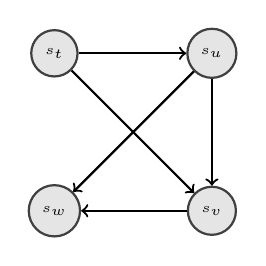
\begin{tikzpicture}
        		\tikzstyle{sentence}=[circle,thick,draw=black!75,fill=black!10,minimum size=2mm]
        		\tikzstyle{edge}=[draw, thick, ->]
       			\begin{scope}
			        \node [sentence] (s1) at (0,2) {\tiny{$s_t$}};
			        \node [sentence] (s2) at (2,2) {\tiny{$s_u$}};
			        \node [sentence] (s3) at (2,0) {\tiny{$s_v$}};
			        \node [sentence] (s4) at (0,0) {\tiny{$s_w$}};  
			        \path[edge] (s1) edge [above] node[font=\tiny] {} (s2);
			        \path[edge] (s1) edge [above] node[font=\tiny] {} (s3);
			        \path[edge] (s2) edge [above] node[font=\tiny] {} (s3);
			        \path[edge] (s2) edge [above] node[font=\tiny] {} (s4);
			        \path[edge] (s3) edge [above] node[font=\tiny] {} (s4);
        		\end{scope}        
      		\end{tikzpicture}
			&

			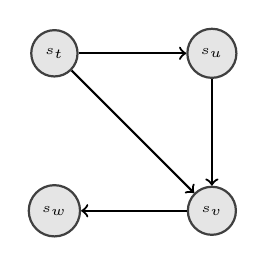
\begin{tikzpicture}
        		\tikzstyle{sentence}=[circle,thick,draw=black!75,fill=black!10,minimum size=2mm]
        		\tikzstyle{edge}=[draw, thick, ->]
       			\begin{scope}
			        \node [sentence] (s1) at (0,2) {\tiny{$s_t$}};
			        \node [sentence] (s2) at (2,2) {\tiny{$s_u$}};
			        \node [sentence] (s3) at (2,0) {\tiny{$s_v$}};
			        \node [sentence] (s4) at (0,0) {\tiny{$s_w$}};  
			        \path[edge] (s1) edge [above] node[font=\tiny] {} (s2);
			        \path[edge] (s1) edge [above] node[font=\tiny] {} (s3);
			        \path[edge] (s2) edge [above] node[font=\tiny] {} (s3);
			        \path[edge] (s3) edge [above] node[font=\tiny] {} (s4);
		        \end{scope}        
	        \end{tikzpicture}
		    \\
		    \scriptsize{$p_1$} & \scriptsize{$p_2$} & \scriptsize{$p_3$} & \scriptsize{$p_4$}
		    \\
		    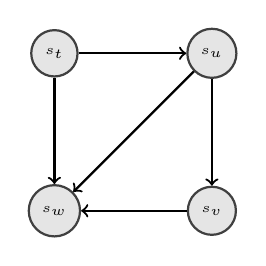
\begin{tikzpicture} 
        		\tikzstyle{sentence}=[circle,thick,draw=black!75,fill=black!10,minimum size=2mm]
        		\tikzstyle{edge}=[draw, thick, ->]
       			\begin{scope}
			        \node [sentence] (s1) at (0,2) {\tiny{$s_t$}};
			        \node [sentence] (s2) at (2,2) {\tiny{$s_u$}};
			        \node [sentence] (s3) at (2,0) {\tiny{$s_v$}};
			        \node [sentence] (s4) at (0,0) {\tiny{$s_w$}};  
			        \path[edge] (s1) edge [above] node[font=\tiny] {} (s2);
			        \path[edge] (s1) edge [above] node[font=\tiny] {} (s4);
			        \path[edge] (s2) edge [above] node[font=\tiny] {} (s3);
			        \path[edge] (s2) edge [above] node[font=\tiny] {} (s4);
			        \path[edge] (s3) edge [above] node[font=\tiny] {} (s4);
        		\end{scope}        
      		\end{tikzpicture}
			&
			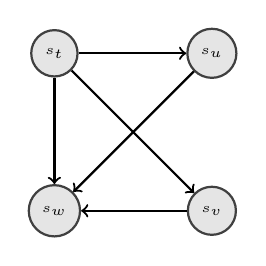
\begin{tikzpicture}
		        \tikzstyle{sentence}=[circle,thick,draw=black!75,fill=black!10,minimum size=2mm]
		        \tikzstyle{edge}=[draw, thick, ->]
		       \begin{scope}
			        \node [sentence] (s1) at (0,2) {\tiny{$s_t$}};
			        \node [sentence] (s2) at (2,2) {\tiny{$s_u$}};
			        \node [sentence] (s3) at (2,0) {\tiny{$s_v$}};
			        \node [sentence] (s4) at (0,0) {\tiny{$s_w$}};  
			        \path[edge] (s1) edge [above] node[font=\tiny] {} (s2);
			        \path[edge] (s1) edge [above] node[font=\tiny] {} (s3);
			        \path[edge] (s1) edge [above] node[font=\tiny] {} (s4);
			        \path[edge] (s2) edge [above] node[font=\tiny] {} (s4);
			        \path[edge] (s3) edge [above] node[font=\tiny] {} (s4);
       			 \end{scope}        
      		\end{tikzpicture}
			&
			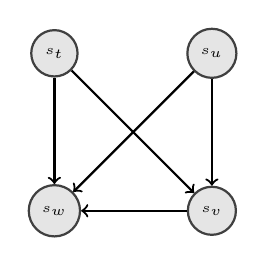
\begin{tikzpicture}
        		\tikzstyle{sentence}=[circle,thick,draw=black!75,fill=black!10,minimum size=2mm]
        		\tikzstyle{edge}=[draw, thick, ->]
       			\begin{scope}
        			\node [sentence] (s1) at (0,2) {\tiny{$s_t$}};
        			\node [sentence] (s2) at (2,2) {\tiny{$s_u$}};
        			\node [sentence] (s3) at (2,0) {\tiny{$s_v$}};
        			\node [sentence] (s4) at (0,0) {\tiny{$s_w$}};  
        			\path[edge] (s1) edge [above] node[font=\tiny] {} (s3);
        			\path[edge] (s1) edge [above] node[font=\tiny] {} (s4);
        			\path[edge] (s2) edge [above] node[font=\tiny] {} (s3);
        			\path[edge] (s2) edge [above] node[font=\tiny] {} (s4);
        			\path[edge] (s3) edge [above] node[font=\tiny] {} (s4);
        		\end{scope}        
      		\end{tikzpicture}
			&
			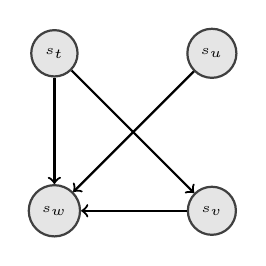
\begin{tikzpicture} 
        		\tikzstyle{sentence}=[circle,thick,draw=black!75,fill=black!10,minimum size=2mm]
        		\tikzstyle{edge}=[draw, thick, ->]
       			\begin{scope}
        			\node [sentence] (s1) at (0,2) {\tiny{$s_t$}};
        			\node [sentence] (s2) at (2,2) {\tiny{$s_u$}};
        			\node [sentence] (s3) at (2,0) {\tiny{$s_v$}};
        			\node [sentence] (s4) at (0,0) {\tiny{$s_w$}};  
        			\path[edge] (s1) edge [above] node[font=\tiny] {} (s3);
        			\path[edge] (s1) edge [above] node[font=\tiny] {} (s4);
        			\path[edge] (s2) edge [above] node[font=\tiny] {} (s4);
        			\path[edge] (s3) edge [above] node[font=\tiny] {} (s4);
        		\end{scope}        
      		\end{tikzpicture}
      		\\

		    \scriptsize{$p_5$} & \scriptsize{$p_6$} & \scriptsize{$p_7$} & \scriptsize{$p_8$}
			\\
			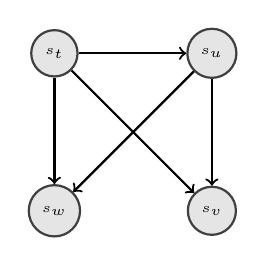
\begin{tikzpicture}
		    	\tikzstyle{sentence}=[circle,thick,draw=black!75,fill=black!10,minimum size=2mm]
		       	\tikzstyle{edge}=[draw, thick, ->]
		       	\begin{scope}
		        	\node [sentence] (s1) at (0,2) {\tiny{$s_t$}};
		        	\node [sentence] (s2) at (2,2) {\tiny{$s_u$}};
		        	\node [sentence] (s3) at (2,0) {\tiny{$s_v$}};
		        	\node [sentence] (s4) at (0,0) {\tiny{$s_w$}};  
		        	\path[edge] (s1) edge [above] node[font=\tiny] {} (s2);
		        	\path[edge] (s1) edge [above] node[font=\tiny] {} (s3);
		        	\path[edge] (s1) edge [above] node[font=\tiny] {} (s4);
		        	\path[edge] (s2) edge [above] node[font=\tiny] {} (s3);
		        	\path[edge] (s2) edge [above] node[font=\tiny] {} (s4);
		        \end{scope}        
		    \end{tikzpicture}
			&
			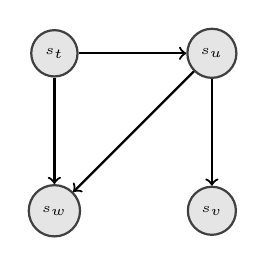
\begin{tikzpicture}
		    	\tikzstyle{sentence}=[circle,thick,draw=black!75,fill=black!10,minimum size=2mm]
		        \tikzstyle{edge}=[draw, thick, ->]
		        \begin{scope}
			        \node [sentence] (s1) at (0,2) {\tiny{$s_t$}};
			        \node [sentence] (s2) at (2,2) {\tiny{$s_u$}};
			        \node [sentence] (s3) at (2,0) {\tiny{$s_v$}};
			        \node [sentence] (s4) at (0,0) {\tiny{$s_w$}};  
			        \path[edge] (s1) edge [above] node[font=\tiny] {} (s2);
			        \path[edge] (s1) edge [above] node[font=\tiny] {} (s4);
			        \path[edge] (s2) edge [above] node[font=\tiny] {} (s3);
			        \path[edge] (s2) edge [above] node[font=\tiny] {} (s4);
		        \end{scope} 
		    \end{tikzpicture}
 			&
			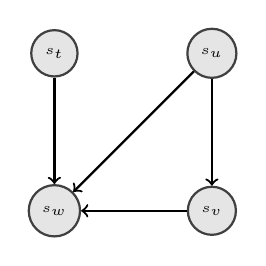
\begin{tikzpicture}
        		\tikzstyle{sentence}=[circle,thick,draw=black!75,fill=black!10,minimum size=2mm]
        		\tikzstyle{edge}=[draw, thick, ->]
       			\begin{scope}
        			\node [sentence] (s1) at (0,2) {\tiny{$s_t$}};
        			\node [sentence] (s2) at (2,2) {\tiny{$s_u$}};
        			\node [sentence] (s3) at (2,0) {\tiny{$s_v$}};
        			\node [sentence] (s4) at (0,0) {\tiny{$s_w$}};  
        			\path[edge] (s1) edge [above] node[font=\tiny] {} (s4);
        			\path[edge] (s2) edge [above] node[font=\tiny] {} (s3);
        			\path[edge] (s2) edge [above] node[font=\tiny] {} (s4);
        			\path[edge] (s3) edge [above] node[font=\tiny] {} (s4);
        		\end{scope}        
      		\end{tikzpicture}
      		&
			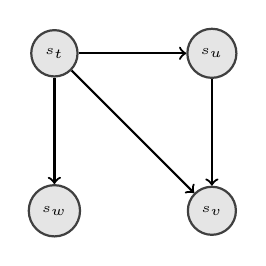
\begin{tikzpicture}
        		\tikzstyle{sentence}=[circle,thick,draw=black!75,fill=black!10,minimum size=2mm]
        		\tikzstyle{edge}=[draw, thick, ->]
       			\begin{scope}
			        \node [sentence] (s1) at (0,2) {\tiny{$s_t$}};
			        \node [sentence] (s2) at (2,2) {\tiny{$s_u$}};
			        \node [sentence] (s3) at (2,0) {\tiny{$s_v$}};
			        \node [sentence] (s4) at (0,0) {\tiny{$s_w$}};  
			        \path[edge] (s1) edge [above] node[font=\tiny] {} (s2);
			        \path[edge] (s1) edge [above] node[font=\tiny] {} (s3);
			        \path[edge] (s1) edge [above] node[font=\tiny] {} (s4);
			        \path[edge] (s2) edge [above] node[font=\tiny] {} (s3);
		        \end{scope}
		    \end{tikzpicture}
			\\

			\scriptsize{$p_9$} & \scriptsize{$p_{10}$} & \scriptsize{$p_{11}$} & \scriptsize{$p_{12}$}
			\\
			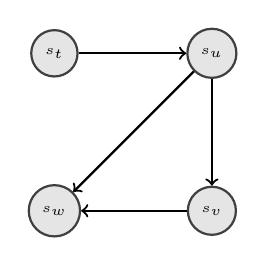
\begin{tikzpicture}
        		\tikzstyle{sentence}=[circle,thick,draw=black!75,fill=black!10,minimum size=2mm]
        		\tikzstyle{edge}=[draw, thick, ->]
       			\begin{scope}
       				\node [sentence] (s1) at (0,2) {\tiny{$s_t$}};
        			\node [sentence] (s2) at (2,2) {\tiny{$s_u$}};
        			\node [sentence] (s3) at (2,0) {\tiny{$s_v$}};
        			\node [sentence] (s4) at (0,0) {\tiny{$s_w$}};  
        			\path[edge] (s1) edge [above] node[font=\tiny] {} (s2);
        			\path[edge] (s2) edge [above] node[font=\tiny] {} (s3);
        			\path[edge] (s2) edge [above] node[font=\tiny] {} (s4);
        			\path[edge] (s3) edge [above] node[font=\tiny] {} (s4);
        		\end{scope}        
      		\end{tikzpicture}
			&
			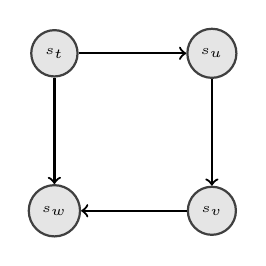
\begin{tikzpicture}
        		\tikzstyle{sentence}=[circle,thick,draw=black!75,fill=black!10,minimum size=2mm]
        		\tikzstyle{edge}=[draw, thick, ->]
       			\begin{scope}
        			\node [sentence] (s1) at (0,2) {\tiny{$s_t$}};
         			\node [sentence] (s2) at (2,2) {\tiny{$s_u$}};
        			\node [sentence] (s3) at (2,0) {\tiny{$s_v$}};
			        \node [sentence] (s4) at (0,0) {\tiny{$s_w$}};  
			        \path[edge] (s1) edge [above] node[font=\tiny] {} (s2);
			        \path[edge] (s1) edge [above] node[font=\tiny] {} (s4);
			        \path[edge] (s2) edge [above] node[font=\tiny] {} (s3);
			        \path[edge] (s3) edge [above] node[font=\tiny] {} (s4);
        		\end{scope}        
      		\end{tikzpicture}
			&
			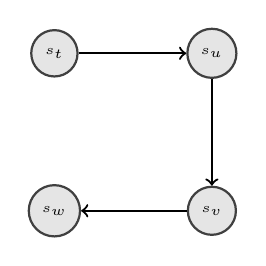
\begin{tikzpicture}
        		\tikzstyle{sentence}=[circle,thick,draw=black!75,fill=black!10,minimum size=2mm]
        		\tikzstyle{edge}=[draw, thick, ->]
       			\begin{scope}
			        \node [sentence] (s1) at (0,2) {\tiny{$s_t$}};
			        \node [sentence] (s2) at (2,2) {\tiny{$s_u$}};
			        \node [sentence] (s3) at (2,0) {\tiny{$s_v$}};
			        \node [sentence] (s4) at (0,0) {\tiny{$s_w$}};  
			        \path[edge] (s1) edge [above] node[font=\tiny] {} (s2);
			        \path[edge] (s2) edge [above] node[font=\tiny] {} (s3);
			        \path[edge] (s3) edge [above] node[font=\tiny] {} (s4);
        		\end{scope}        
      		\end{tikzpicture}
			&
			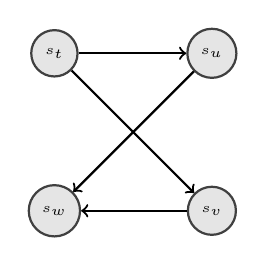
\begin{tikzpicture}
       			\tikzstyle{sentence}=[circle,thick,draw=black!75,fill=black!10,minimum size=2mm]
        		\tikzstyle{edge}=[draw, thick, ->]
       			\begin{scope}
        			\node [sentence] (s1) at (0,2) {\tiny{$s_t$}};
        			\node [sentence] (s2) at (2,2) {\tiny{$s_u$}};
        			\node [sentence] (s3) at (2,0) {\tiny{$s_v$}};
        			\node [sentence] (s4) at (0,0) {\tiny{$s_w$}};  
        			\path[edge] (s1) edge [above] node[font=\tiny] {} (s2);
        			\path[edge] (s1) edge [above] node[font=\tiny] {} (s3);
        			\path[edge] (s2) edge [above] node[font=\tiny] {} (s4);
        			\path[edge] (s3) edge [above] node[font=\tiny] {} (s4);
        		\end{scope}        
      		\end{tikzpicture}
			\\

			\scriptsize{$p_{13}$} & \scriptsize{$p_{14}$} & \scriptsize{$p_{15}$} & \scriptsize{$p_{16}$}
			\\
			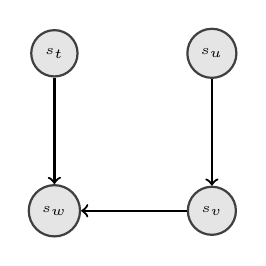
\begin{tikzpicture}
        		\tikzstyle{sentence}=[circle,thick,draw=black!75,fill=black!10,minimum size=2mm]
        		\tikzstyle{edge}=[draw, thick, ->]
       			\begin{scope}
			        \node [sentence] (s1) at (0,2) {\tiny{$s_t$}};
			        \node [sentence] (s2) at (2,2) {\tiny{$s_u$}};
			        \node [sentence] (s3) at (2,0) {\tiny{$s_v$}};
			        \node [sentence] (s4) at (0,0) {\tiny{$s_w$}};  
			        \path[edge] (s1) edge [above] node[font=\tiny] {} (s4);
			        \path[edge] (s2) edge [above] node[font=\tiny] {} (s3);
			        \path[edge] (s3) edge [above] node[font=\tiny] {} (s4);
        		\end{scope}       
      		\end{tikzpicture}
      		&
			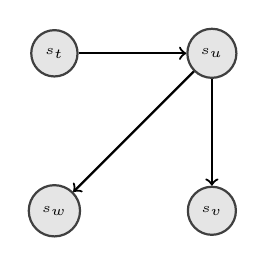
\begin{tikzpicture}
        		\tikzstyle{sentence}=[circle,thick,draw=black!75,fill=black!10,minimum size=2mm]
        		\tikzstyle{edge}=[draw, thick, ->]
		        \begin{scope}
			        \node [sentence] (s1) at (0,2) {\tiny{$s_t$}};
			        \node [sentence] (s2) at (2,2) {\tiny{$s_u$}};
			        \node [sentence] (s3) at (2,0) {\tiny{$s_v$}};
			        \node [sentence] (s4) at (0,0) {\tiny{$s_w$}};  
			        \path[edge] (s1) edge [above] node[font=\tiny] {} (s2);
			        \path[edge] (s2) edge [above] node[font=\tiny] {} (s3);
			        \path[edge] (s2) edge [above] node[font=\tiny] {} (s4);
		        \end{scope}        
	        \end{tikzpicture}
			&
			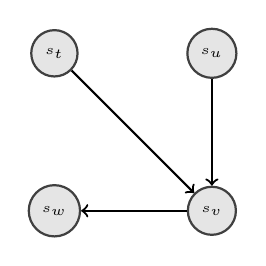
\begin{tikzpicture}
        		\tikzstyle{sentence}=[circle,thick,draw=black!75,fill=black!10,minimum size=2mm]
        		\tikzstyle{edge}=[draw, thick, ->]
       			\begin{scope}
         			\node [sentence] (s1) at (0,2) {\tiny{$s_t$}};
         			\node [sentence] (s2) at (2,2) {\tiny{$s_u$}};
        			\node [sentence] (s3) at (2,0) {\tiny{$s_v$}};
        			\node [sentence] (s4) at (0,0) {\tiny{$s_w$}};  
        			\path[edge] (s1) edge [above] node[font=\tiny] {} (s3);
        			\path[edge] (s2) edge [above] node[font=\tiny] {} (s3);
        			\path[edge] (s3) edge [above] node[font=\tiny] {} (s4);
        		\end{scope}        
      		\end{tikzpicture}
			&
			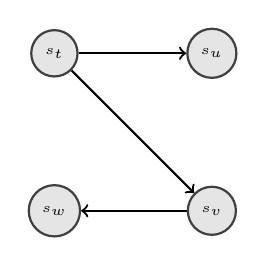
\begin{tikzpicture}
        		\tikzstyle{sentence}=[circle,thick,draw=black!75,fill=black!10,minimum size=2mm]
        		\tikzstyle{edge}=[draw, thick, ->]
       			\begin{scope}
			        \node [sentence] (s1) at (0,2) {\tiny{$s_t$}};
			        \node [sentence] (s2) at (2,2) {\tiny{$s_u$}};
			        \node [sentence] (s3) at (2,0) {\tiny{$s_v$}};
			        \node [sentence] (s4) at (0,0) {\tiny{$s_w$}};  
			        \path[edge] (s1) edge [above] node[font=\tiny] {} (s3);
			        \path[edge] (s1) edge [above] node[font=\tiny] {} (s2);
			        \path[edge] (s3) edge [above] node[font=\tiny] {} (s4);
			    \end{scope}        
     		\end{tikzpicture}
			\\
			\scriptsize{$p_{17}$} & \scriptsize{$p_{18}$} & \scriptsize{$p_{19}$} & \scriptsize{$p_{20}$}
			
			\\
			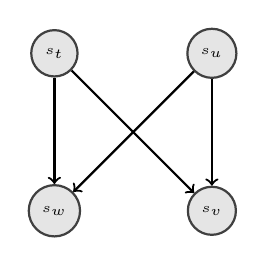
\begin{tikzpicture}
			    \tikzstyle{sentence}=[circle,thick,draw=black!75,fill=black!10,minimum size=2mm]
			    \tikzstyle{edge}=[draw, thick, ->]
			    \begin{scope}
			        \node [sentence] (s1) at (0,2) {\tiny{$s_t$}};
			        \node [sentence] (s2) at (2,2) {\tiny{$s_u$}};
			        \node [sentence] (s3) at (2,0) {\tiny{$s_v$}};
			        \node [sentence] (s4) at (0,0) {\tiny{$s_w$}};  
			        \path[edge] (s1) edge [above] node[font=\tiny] {} (s3);
			        \path[edge] (s1) edge [above] node[font=\tiny] {} (s4);
			        \path[edge] (s2) edge [above] node[font=\tiny] {} (s3);
			        \path[edge] (s2) edge [above] node[font=\tiny] {} (s4);
			    \end{scope}        
			\end{tikzpicture}
			&
			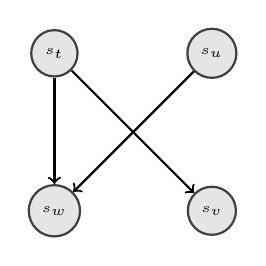
\begin{tikzpicture}
        		\tikzstyle{sentence}=[circle,thick,draw=black!75,fill=black!10,minimum size=2mm]
        		\tikzstyle{edge}=[draw, thick, ->]
        		\begin{scope}
        			\node [sentence] (s1) at (0,2) {\tiny{$s_t$}};
				    \node [sentence] (s2) at (2,2) {\tiny{$s_u$}};
				    \node [sentence] (s3) at (2,0) {\tiny{$s_v$}};
				    \node [sentence] (s4) at (0,0) {\tiny{$s_w$}};  
				    \path[edge] (s1) edge [above] node[font=\tiny] {} (s3);
				    \path[edge] (s1) edge [above] node[font=\tiny] {} (s4);
				    \path[edge] (s2) edge [above] node[font=\tiny] {} (s4);
        		\end{scope}        
      		\end{tikzpicture}
      		&
			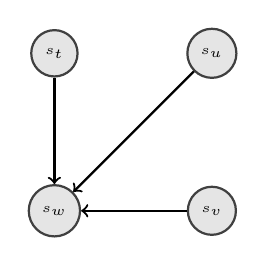
\begin{tikzpicture}
        		\tikzstyle{sentence}=[circle,thick,draw=black!75,fill=black!10,minimum size=2mm]
        		\tikzstyle{edge}=[draw, thick, ->]
       			\begin{scope}
			        \node [sentence] (s1) at (0,2) {\tiny{$s_t$}};
			        \node [sentence] (s2) at (2,2) {\tiny{$s_u$}};
			        \node [sentence] (s3) at (2,0) {\tiny{$s_v$}};
			        \node [sentence] (s4) at (0,0) {\tiny{$s_w$}};  
			        \path[edge] (s1) edge [above] node[font=\tiny] {} (s4);
			        \path[edge] (s2) edge [above] node[font=\tiny] {} (s4);
			        \path[edge] (s3) edge [above] node[font=\tiny] {} (s4);
        		\end{scope}        
      		\end{tikzpicture}
      		&
			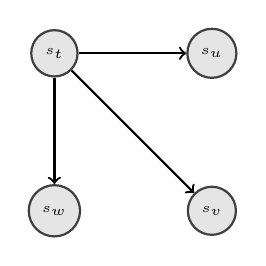
\begin{tikzpicture}
        		\tikzstyle{sentence}=[circle,thick,draw=black!75,fill=black!10,minimum size=2mm]
        		\tikzstyle{edge}=[draw, thick, ->]
       			\begin{scope}
			        \node [sentence] (s1) at (0,2) {\tiny{$s_t$}};
			        \node [sentence] (s2) at (2,2) {\tiny{$s_u$}};
			        \node [sentence] (s3) at (2,0) {\tiny{$s_v$}};
			        \node [sentence] (s4) at (0,0) {\tiny{$s_w$}};  
			        \path[edge] (s1) edge [above] node[font=\tiny] {} (s2);
			        \path[edge] (s1) edge [above] node[font=\tiny] {} (s3);
			        \path[edge] (s1) edge [above] node[font=\tiny] {} (s4);
        		\end{scope}        
      		\end{tikzpicture}
      		\\
      		\scriptsize{$p_{21}$} & \scriptsize{$p_{22}$} & \scriptsize{$p_{23}$} & \scriptsize{$p_{24}$}
		\end{tabular}
		}%
	\end{center}
	\caption{Coherence patterns with four nodes where $t<u<v<w$.}
	\label{fig:4node-patterns}
\end{figure}


\paragraph{Results.}

Given the extracted coherence patterns as basis graphs, we compute the graph signature representation of each projection graph corresponding with each text in the dataset. 
The elements of the graph signature of a projection graph are frequencies of the extracted patterns in the projection graph. 
These elements together model the connectivity style of the graph. 
From the texture perspective, the frequency of each subgraph models how frequently a coherence pattern occurs in a text. 

We begin with the evaluation of the average outdegree metric as proposed by the entity graph model. 
Table \ref{tab:correlation-outdegree} shows the results of computing the Pearson correlation between the average outdegree of three projection graphs defined in the entity graph model \cite{guinaudeau13}. 
Each row of the table presents the type of the projection graph that is used (see Chapter \ref{ch:rel-work}) to represent texts. 
The column with header $\rho$ contains the coefficient of the Pearson correlation, and p\_value is what we use to identify significant correlations. 
The results show that the average outdegree of none of the projection graphs is significantly correlated with ratings assigned by humans, confirming our argument at the beginning of this section:  The average outdegree metric is insufficient to capture the connectivity style of graphs, and therefore the coherence of a text. 

\begin{table}[!ht]
	\begin{center}
		\begin{tabular}{lcc}
			\toprule
 			\textbf{Projection type}& $\boldsymbol\rho$  & \textbf{P\_value}\\
 			\midrule
			$P_U$ 				& $-0.013$ 						& $0.949$ \\
			$P_W$ 				& $\textcolor{white}{+}0.151$  	& $0.452$ \\
			$P_{Acc}$ 			& $\textcolor{white}{+}0.150$ 	& $0.455$ \\
			\bottomrule
		\end{tabular}
	\end{center}
	\caption{The correlation of the average outdegree metric of different projection graphs with readability ratings assigned by human judges.}
 	\label{tab:correlation-outdegree}
\end{table}


Table \ref{tab:correlation-3node} shows the Pearson correlation coefficient and their corresponding p\_value between the frequencies of 3-node coherence patterns (see Figure \ref{fig:3node-patterns}) and readability ratings assigned by human judges. 

\begin{table}[!ht]
	\begin{center}
		\begin{tabular}{lcc}
		\toprule
  	 	\textbf{3-node patterns} & $\boldsymbol\rho$ 		& \textbf{P\_value}	 \\
  	 	\midrule
 		$p_1$ 			& $\textcolor{white}{+}0.310$ & $0.116$ 		\\
 		$p_2$ 			& $-0.325$ 				      & $0.098$ 		\\
		$\mathbf{p_3}$ 	& $\mathbf{-0.384}$ 		  & $\mathbf{0.048}$\\
 		$p_4$ 			& $\textcolor{white}{+}0.108$ & $0.592$			\\
 		\bottomrule
		\end{tabular}
	\end{center}
	\caption{The Pearson correlation coefficient and p\_value between the frequency of \mbox{3-node} patterns (see Figure \ref{fig:3node-patterns}) and readability ratings assigned by human judges.} 
 	\label{tab:correlation-3node}
\end{table}

The results presented in Table \ref{tab:correlation-3node} show that the frequencies of pattern $p_1$ and pattern $p_4$ are positively and the frequencies of pattern $p_2$ and pattern $p_3$ are negatively correlated with readability ratings. 
Among them, the frequency of pattern $p_3$ significantly correlates with human readability rankings. 
This pattern is similar to the shift in the center among sentences in a text. 
Since we are computing the frequency of this pattern in each text, this result shows that texts with many shifts in the center are perceived challenging to read. 
We notice that the frequency of pattern $p_1$ is positively correlated with readability rankings, not significantly though. 
This shows that this pattern occurs many times in easy to read texts.  
This pattern captures a sentence that introduces some information, which is limited in our model to entities, then subsequent sentences are about that information. 
These results are compatible with the structure of paragraphs in news articles. 
Good writers usually initiate topics, ideas or claims and then provide clear elaboration and reasons. 
%That is, a sequence of many related words and phrases will be evoked to explain an idea provide an account of the writer's reasoning. 
Also, in English-speaking schools of essay writing and debating, there is the tendency to state the central claim of a text or a paragraph in the very first sentence followed by supporting arguments \cite{peldszus15}. 

The frequency of pattern $p_2$ negatively correlates with human rankings, showing that this pattern has not been observed in coherent texts as frequently as in incoherent ones. 
This explains that it is difficult for readers to process sentences that become connected via their following sentences.  
Interestingly, the structural difference between pattern $p_2$ and pattern $p_1$ can be interpreted as the difference in the order of sentences. 
If node $s_t$ proceeded node $s_u$ in pattern $p_2$ then this pattern would look like pattern $p_1$, which is a property of coherent texts. 
This means that these patterns can capture the order of information presented in sentences as well. 

Finally, the frequency of one of our coherence patterns, unlike the average outdegree, is significantly correlated with human readability ratings. 
The correlation coefficients, $\rho$, have more distance to zero in comparison to those of the average outdegree metric. 
It indicates that the frequency of coherence patterns is more correlated with readability scores assigned by human judges compared to the average outdegree.  
Coherence patterns capture the connectivity style among sentences in a text as small units and beyond individual sentence connectivities.
It is one of the essential differences between our coherence patterns and average outdegree. 

Table \ref{tab:correlation-4node} shows the Pearson correlation coefficient and their corresponding p\_value between the frequencies of 4-node patterns and readability ratings assigned by human judges. 
Although patterns have the same number of nodes, they may contain a different number of edges. 
The second column presents the number of edges in each pattern. 

\begin{table}[!ht]
	\begin{center}
		\begin{tabular}{lccc}
			\toprule
   			\textbf{4-node patterns}& \textbf{Number of edges} & $\boldsymbol\rho$ 		& \textbf{P\_value}				\\
   			\midrule
			$p_1$ 				& 6 			  & $\textcolor{white}{+}{0.103}$ 	& $0.609$					\\
			$p_2$ 				& 5 			  & $-0.212$ 					 	& $0.288$					\\
			$p_3$  				& 5				  & $-0.176$				     	& $0.380$					\\
			$p_4$  				& 4 			  & $-0.257$ 				     	& $0.196$					\\
			$p_5$ 				& 5 			  & $-0.140$ 					 	& $0.486$					\\
			$p_6$  				& 5 			  & $\textcolor{white}{+}{0.200}$  	& $0.317$					\\
			$\mathbf{p_7}$ 	& \textbf{5} 	  & $\mathbf{-0.402}$ 			 	& $\mathbf{0.038}$			\\
			$p_8$  				& 4 			  & $-0.317$ 					 	& $0.107$					\\
			$p_9$ 				& 5 			  & $\textcolor{white}{+}{0.153}$  	& $0.446$					\\
			$p_{10}$ 			& 4 			  & $-0.238$ 					 	& $0.232$					\\
			$\mathbf{p_{11}}$ 	& \textbf{4} 	  & $\mathbf{-0.509}$            	& $\mathbf{0.007}$			\\
			$\mathbf{p_{12}}$  	& \textbf{4} 	  & $\mathbf{\textcolor{white}{+}{0.449}}$ & $\mathbf{0.019}$	\\
			$p_{13}$			& 4 			  & $-0.045$ 						& $0.824$					\\
			$p_{14}$			& 4 			  & $-0.033$ 						& $0.870$					\\
			$p_{15}$			& 3				  & $-0.358$ 						& $0.067$					\\
			$p_{16}$ 			& 4 			  & $-0.068$ 						& $0.736$					\\
			$p_{17}$			& 3 			  & $-0.308$ 						& $0.118$					\\
			$\mathbf{p_{18}}$	& \textbf{3}	  & $\mathbf{-0.546}$				& $\mathbf{0.003}$			\\
			$\mathbf{p_{19}}$	& \textbf{3} 	  & $\mathbf{-0.601}$ 				& $\mathbf{0.001}$			\\
			$p_{20}$			& 3 			  & $\textcolor{white}{+}{0.094}$   & $0.641$					\\
			$p_{21}$			& 4 			  & $\textcolor{white}{+}{0.068}$	& $0.736$				    \\
			$p_{22}$			& 3				  & $-0.374$ 						& $0.055$					\\
			$p_{23}$			& 3				  & $-0.314$ 						& $0.111$					\\
			$p_{24}$ 			& 3				  & $\textcolor{white}{+}{0.100}$   & $0.620$					\\
			\bottomrule
		\end{tabular}
	\end{center}
	\caption{The number of edges in 4-node patterns, and the Pearson correlation coefficient and their corresponding p\_value between the frequency of patterns and human-provided readability ratings.} 
	\label{tab:correlation-4node}
\end{table}

Among all patterns that have positive correlation coefficients with readability scores, $p_{12}$ has the highest correlation coefficient. 
In contrast, the most negative correlation coefficient is for pattern $p_{11}$. 
A comparison of these two patterns shows that they have the same number of edges but different styles of connectivity.
This confirms our intuitions: (i) The connectivity structure of projection graphs that represent coherent texts are similar to each other and different from those that represent incoherent texts. 
(ii) The frequency of subgraphs can encode the connectivity structure of projection graphs and consequently coherence. 
Moreover, these patterns roughly remind us of the \emph{ambiguity node}\ phenomenon introduced by \newcite{stoddard91} [p.\ 29]: 
\emph{
    ``[...] in some cases, there may be more than one logical, possible node for a given cohesive element in a text, in which case, a reader may see the resulting ambiguity but not be able to decide between the choices''.
    }
In pattern $p_{11}$ a reader may need to make a decision about the center in $s_w$, whereas in $p_{12}$ the center of $s_w$ is the same as the center of $s_t$. 
This phenomenon can also be observed in all positively correlated patterns.  
It can be interpreted such that if readers have to return to one point in the text, they prefer to return to a sentence which is the core of the preceding sentences.

With reference to the results related to 3-node patterns, presented in Table \ref{tab:correlation-3node}, and the results of 4-node patterns, shown in Table \ref{tab:correlation-4node}, two observations are noticeable. 
First, the correlation coefficients of the 4-node patterns that are significantly correlated with readability ratings are stronger, which means their absolute value is higher, than those of 3-node patterns. 
This confirms our intuition that large subgraphs capture more information about the connectivity style of projection graphs. 
So, they are potent predictors of coherence in comparison to 3-node patterns. 
Second, the correlation coefficient obtained for pattern $p_{12}$, as the pattern with the strongest correlation, in 4-node patterns is greater than the correlation coefficient of pattern $p_4$, as the pattern with the strongest correlation, in 3-node patterns. 
This can be because $p_{12}$ captures more circumstances about the connectivity of node $s_t$. 
However, we should refrain from interpreting too much into these patterns. 

Finally, \newcite{pitler08} show that none of the entity transition features of the entity grid coherence model strongly correlate with readability ratings of these texts. 
While these features intend to capture entity-based coherence, they seem to be too weak to do so in isolation. 
In contrast to \newcite{pitler08}, we are able to report a statistically significant correlation between some entity-based features and human readability ratings.

We summarize our observations in this experiment as follows: 

\begin{itemize}

	\item The average outdegree metric proposed by \newcite{guinaudeau13} is not significantly correlated with human ratings assigned to texts in the examined dataset;

	\item 3-node patterns, mined from projection graphs, are roughly similar to patterns introduced by \newcite{danes74a};

	\item The connectivity style of a projection graph can be encoded by the frequency of extracted subgraphs or coherence patterns.

\end{itemize}


\subsubsection{Readability Ranking}

In this experiment, we use coherence models to rank texts with respect to their readability property. 
Given that easier to read texts are more coherent than difficult texts, a coherence model should ideally be able to rank texts with respect to their readability. 
We investigate how thoroughly rankings predicted by a coherence model match rankings that are based on the readability ratings assigned by humans. 
The readability ranking task may in principle be more natural than readability assessment because in most NLP applications the main concern is with the relative quality of texts rather than their absolute scores. 
Following \newcite{pitler08} we rank texts in a pairwise approach with respect to their readability ratings that are assigned by humans. 
We treat this task as a classification task: Given a pair of texts, which one is easier to read or more coherent?

\paragraph{Evaluation Metric.}
The performance of a set of features that capture coherence for the readability ranking task is measured by the accuracy of rankings predicted by the classification model where it is supplied by the feature set. 
The accuracy is calculated as follows:

\begin{equation}
Accuracy = \frac{\textit{the number of correct rankings}}{\textit{the number of pairs}}. 
\end{equation} 

We also compute the F-measure in order to compare our features with baseline features. 
The F-measure is the average of the F1-scores which are computed for each class. 
Note that our problem is ranking which is treated as classification. 
There is no True class to be classified. 
So, in different turns, we take each class as the true class and compute the F1-measure for that class. 
Then we report the average F1-scores as the F-measure for this task. 
The F1-score for each class is the harmonic mean of precision ($P$) and recall $R$:

\begin{equation}
\textit{F1-score} = 2\frac{P \cdot R}{P + R}.  
\end{equation}
Precision is computed as follows: 

\begin{equation}
P = \frac{\textit{the number of correct decisions}}{\textit{the number of decisions}},
\end{equation}
and recall is calculated as follows:

\begin{equation}
R = \frac{\textit{the number of correct decisions}}{\textit{the number of pairs in that class}}.
\end{equation}

Since the dataset is not accompanied by any standard split of training and test sets, we used 10-fold cross-validation for comparing the quality of different coherence feature sets. 
The reported numbers are the average of all numbers obtained from all runs of \mbox{10-fold} \mbox{cross-validation}. 

\paragraph{Experimental settings.}
The settings of this experiment are as it is performed by \newcite{pitler08}. 
Text pairs include texts, from the dataset introduced in Section \ref{sec:data_pitler}, whose readability ratings differ by at least $0.5$. 
This criterion ensures that the difference in readability ratings of texts in a text pair is noticeable enough that a coherence model distinguishes their differences. 
If the first text in a pair has a higher readability score, a label $+1$ is assigned to the pair; otherwise, a label $-1$ is assigned. 
In total, the number of pairs obtained by this procedure is 209 pairs in which 105 pairs have label $+1$, and 104 pairs have label $-1$.  
We employ WEKA's linear support vector implementation (SMO) to classify the pairs.
The SMO model is supplied with different sets of features representing the coherence of each text. 
The first set of features is grammatical transitions of entities, with a sequence length of two, proposed by the entity grid model \cite{barzilay05a,barzilay08}. 
For creating entity grids we use Brown Coherence Toolkit v1.0, which is set up in a docker by the author of this thesis\footnote{The docker is available \url{https://github.com/MMesgar/text_to_entity_grid}} to be used quickly for future research. 
The input parse trees to this toolkit are gold parse trees from Penn TreeBank II \cite{marcus94}. 

\paragraph{Results.}
We compare our graph-based coherence features, which are the frequencies of \mbox{k-node} subgraphs in projection graphs, with the proposed features obtained from grammatical transitions of entities by the entity grid model. 
In order to compare different sets of coherence features, we employ the same machine learning model, i.e. SVM, for training and testing on each feature set. 

Table \ref{tab:ranking-pitler} summarizes the results of the readability ranking task on this dataset. 
Since the reported F-Measure and Accuracy have the same trend, we compare systems only based on Accuracy.  
Baseline features are the frequency of grammatical transitions of entities across sentences. 
This feature set is also evaluated\footnote{The accuracy reported in their paper is $79.42\%$. Our reimplementation achieves higher accuracy because our dataset has three articles less.} as coherence features on this dataset by \newcite{pitler08}.

\begin{table}[!ht]
	\begin{center}
		\begin{tabular}{lcc}
			\toprule
			\textbf{Features} 				  & \textbf{Accuracy}							& \textbf{F-measure}	\\
			\midrule
			None (Majority class) 			  & $47.85\%\onewhitestar$						& $0.478\onewhitestar$		\\
			Baseline features 			  	  & \underline{$83.25\%$}$\onewhitestar$     		& \underline{$0.833$}$\onewhitestar$		\\
			3-node 							  & $79.43\%\onewhitestar$						& $0.794\onewhitestar$		\\
			4-node 						      & $89.00\%^\onestar$							& $0.890^\onestar$		\\
			3-node \& 4-node 				  & $88.52\%^\onestar$							& $0.885^\onestar$		\\
			Baseline features + 4-node 		  & $93.30\%^\onestar$							& $0.933^\onestar$		\\
			\bottomrule
		\end{tabular}
	\end{center}
	\caption{The accuracy of the SMO classifier with different sets of features which represent coherence. $\onestar$ indicates statistically significant ($p_value<.01$) improvements with respect to the baseline.}   
	\label{tab:ranking-pitler}
\end{table}

The accuracy of the classifier where it is supplied with 3-node subgraphs as coherence patterns is lower than where it is supplied by the entity grid's features.   
This could happen because of two reasons. 
The entity grid features represent grammatical role transitions of entities, which is more informative than the connections used in 3-node patterns.
Connections in 3-node patterns only capture the existence of at least one shared entity between sentences. 
On the other hand, 3-node patterns are small and consequently more likely to occur in most projection graphs, so their frequencies cannot distinguish between coherent and incoherent texts effectively. 

The feature set containing the frequency of 4-node patterns outperforms the baseline feature set by about $6\%$ in accuracy. 
This confirms our intuition that the entity-based connectivity structure among sentences, which is modeled by projection graphs, distinguishes coherent texts from incoherent texts. 
An advantage of 4-node patterns over the baseline features is that long-distance relations are also taken into account. 
However, our coherence patterns lack the grammatical information in the entity relations. 
Our other hypothesis was that since 4-node patterns are larger than 3-node patterns, they have more capacity in terms of nodes and edges, to model the connectivity style of projection graphs and therefore coherence. 
 Comparing the accuracy of 4-node patterns against 3-node patterns confirms this hypothesis. 
4-node patterns outperform 3-node patterns by $10\%$ difference in accuracy. 
That is a substantial improvement. 
It also verifies that 4-node patterns capture more information about the connectivity style of projection graphs compared to 3-node patterns.      

We combine the frequency of 3-node and 4-node patterns into one feature set and supply it to the classifier.   
The obtained accuracy is superior to the one with only 3-node patterns but slightly worse  ($-1\%$) than the one with only 4-node patterns. 
An explanation for this is that 4-node patterns implicitly contain 3-node patterns in themselves. 
Combining these two sets of features does not probably provide any useful information for modeling the connectivity style of projection graphs more than what exists in 4-node patterns. 

Finally, the combination of baseline features, i.e.\ the frequency of grammatical transitions of entities over adjacent sentences, and 4-node subgraphs achieves the best accuracy. 
An interpretation for this is that although our coherence patterns capture the connectivity structure among sentences of a text, integrating linguistic information such as syntactic transitions of entities may improve the quality of a coherence model.  

\subsection{Automatic Summarization}
\label{sec:auto-summarization}

In this section, we evaluate our approach to coherence pattern mining in automatic text summarization, which is an instance of text generation tasks.  
We employ the summarization system proposed by \newcite{parveen15a} as it is developed on the entity graph model (see Chapter \ref{ch:rel-work}). 
This matters because the entity graph model is the framework of our coherence model as well.  
\newcite{parveen15a} assume that the outdegree of a node in the projection graph of an input text measures how severe its corresponding sentence is for the coherence of the summary.  
This assumption has three weaknesses: 

\begin{itemize}
	\item 
    The summarizer becomes biased to extract sentences from the beginning of a text because these sentences potentially have high outdegrees. 
    This is because edges in a projection graph are directed to capture the sentence order in a text.
    As the text progresses, the potential outdegrees of sentence nodes decrease. 
    As an example, assume a text with $n$ sentences, the outdegree of the first sentence in this text can be high as up to $n-1$, but the outdegree of the last sentence is zero. 
    It is worth mentioning that in the entity graph coherence model, the outdegrees of nodes in a projection graph are averaged to measure the connectivity of the graph or the coherence of the entire text.  
    Limiting this metric to each sentence node does not imply that the sentence is crucial for the coherence of the summary of the text.   
	
	\item 
    In the summarization model proposed by \newcite{parveen15a}  the outdegrees of sentence nodes are computed in the projection graph of the input text.   
    The ideal aim of a summarization system is to extract sentences that make the summary coherent. 
    So, the connectivity of sentences should be evaluated concerning only selected sentences for the summary, rather than all sentences in the input text. 


	\item In the readability experiment in the previous section, we have shown that the average outdegree is not the best metric for encoding the connectivity style of projection graphs and therefore coherence. 
	
\end{itemize} 

We focus on the coherence aspect of the summarization system proposed by \newcite{parveen15a} with two motivations: to use the automatic summarization task as another application for evaluating our graph-based coherence patterns; and to improve the performance of the examined summarization model by integrating our coherence patterns, rather than outdegree, into the summarization model. 
Our intuition is that human-generated summaries given in a dataset are expected to be coherent enough to be readable.
So, if a summarization system extracts sentences of a text so that their connectivity style in the produced summary is similar to the connectivity style of sentences in human-generated summaries, then the produced summary is sufficiently well-connected and therefore coherent. 

\paragraph{Summarization Problem Formulation.}
We use the notation $H$ to denote a dataset which consists of summaries written by humans for a set of texts.  
We use another dataset consisting of a set of document-summary pairs where the $i$th pair contains document $d_i$ and its gold summary $s_i$ written by humans, which is represented by $D=\lbrace \left( d_0, s_0 \right), \left( d_1, s_1 \right),...,\left( d_N, s_N \right) \rbrace$. 
Parameter $N$ is the number of document-summary pairs.  
We assume that each document has a title. 
In practice, in automatic summarization models when an input text does not have any title, the first sentence of the text is taken as the title. 
Gold summaries can be employed to train a summarization model, and can also be used to evaluate summaries produced by the model during the evaluation phase. 
We make a challenging assumption such that documents in $H$ and $D$ are disjoint (i.e.\ there is no intersection among summaries or documents of these two datasets) but come from the same genre. 

\subsubsection{Coherence Pattern Mining}
Here we explain how our coherence patterns are integrated into the summarizer proposed by \newcite{parveen15a}. 
We extract all coherence patterns from the human summaries that are collected in $H$. 
To this end, we represent all texts in this dataset by their entity graph representations. 
Then we apply one-mode projection $P_U$ to entity graphs for obtaining projection graphs. 
We refer to the set of projection graphs that represent texts in $H$ by $GS_H$, which stands for the Graph Set of H. 
Afterward, we use the gSpan method to extract all possible subgraphs from graphs in $GS_H$. 
In Section \ref{sec:readability_assessment}, we have shown that frequencies of coherence patterns in a projection graph capture the connectivity style of the graph and correlate with readability ratings assigned by humans.  
Similarly, we take the subgraphs that frequently occur in $GS_H$ as the connectivity styles that are desired by humans to connect sentences in summaries. 
In order to model this, we weight each coherence pattern based on its number of occurrences, i.e.\ count, in graphs in $GS_H$.  
The weight of a coherence pattern, $weight(p_u)$, is the sum of its counts in all graphs in $GS_H$ divided by its maximum count:

\begin{equation}
\label{eq:ch-weight}
weight(p_u) = \frac{\sum_{k=1}^{M}{count(p_u,g_k)}}{\max_{k=1}^{M}{count(p_u,g_k)}},
\end{equation}
where $M$ is the number of graphs in $GS_H$, and $g_k$ indicates the $k$th projection graph in $GS_H$.
The nominator of the weight function is the sum of the number of occurrences of pattern $p_u$ in graphs in $GS_H$. 
The denominator diminishes the weight of a coherence pattern if it occurs in a few graphs of $GS_H$. 
In an extreme case, if a pattern occurs only in one graph in the graph set then $max_{k=1}^{q}{count(p_u,g_k)}$ is equal to $\sum_{k=1}^{q}{count(p_u,g_k)}$, so the weight of the pattern becomes one. 
If a pattern occurs in many graphs in $GS_H$ the denominator becomes smaller than the nominator; therefore the weight becomes greater than one. 
The weights of coherence patterns are not on the same scale.  
So we normalize the weights by 

\begin{equation}
z = \frac{x-\mu}{\sigma},
\end{equation}
where $\mu$ and $\sigma$ respectively are the mean and the standard deviation of all weights. Variable $x$ is the weight of a pattern.   
Finally a sigmoid function
\begin{equation}
 g(z) = \frac{1}{1+exp(-z)},
\end{equation}
scales weights to a value between $0$ and $1$. 

\subsubsection{Summary Generation}

Assume that we want to produce a summary for document $d$ from dataset $D$. 
\newcite{parveen15a} develop an Integer Linear Programming (ILP) approach to extract the best possible subset of sentences with respect to importance, non-redundancy and coherence factors. 
They measure the contribution of each sentence in a document to the coherence of the output summary by the outdegree of the sentence node in the projection graph representation of the input text.  
To formulate the problem in ILP we represent all sentences in input document $d$ by set 
$S = \lbrace \hat{s}_0, \hat{s}_1,..., \hat{s}_n \rbrace$, where $\hat{s}_i$ is a boolean variable whose value represents if the $i$th sentence of document $d$ is selected for the summary or not.  
Set $E=\lbrace \hat{e}_1, \hat{e}_2,..., \hat{e}_m \rbrace$ is a set of boolean variables representing entities in a text. 
The value of variable $\hat{e}_i$ represents if its associated entity is mentioned in the selected sentences or not. 
Set $P= \lbrace \hat{p}_1, \hat{p}_2,..., \hat{p}_k \rbrace$ is a set of boolean variables which are associated with coherence patterns. 
The True value of a variable in this set indicates that the pattern associated with the variable is a subgraph in the projection graph of the generated summary. 
We consider different weights, i.e.\ $\lambda_I$, $\lambda_R$, and $\lambda_C$, for the significant factors of a good summary, i.e.,\ importance, non-redundancy, and pattern-based coherence.  
The objective function of ILP is as follows: 

\begin{equation}
\max(\lambda_I f_I(S) + \lambda_R f_R(E) + \lambda_C f_C(P)),
\end{equation}
where $f_I(S)$ is the function that measures the importance of the selected sentences, $f_R(E)$ measures the redundancy among the selected sentences with respect to the selected entities, and $f_C(P)$ measures the coherence of the selected sentences with respect to coherence patterns extracted from dataset $H$. 

The importance function, $f_I(S)$, is calculated by considering the ranks of selected sentences for a summary:

\begin{equation}
f_I(S) = \sum_{i=1}^{n}{Rank(s_i) \cdot \hat{s}_i},
\end{equation}
where $Rank(s_i)$ represents the rank of sentence $s_i$ compared to other sentences. 
Parameter $n$ is the number of sentences in input document $d$.  

The ranks of sentences are calculated by the \mbox{Hyperlink-Induced} Topic Search (HITS) algorithm.
The HITS algorithm was developed by \newcite{kleinberg99} for ranking web pages considering the way they are connected.  
\newcite{kleinberg99} categorized web pages into two groups:  Authorities, which are informative web pages; and Hubs, pages that link to informative web pages\footnote{The idea behind Hubs and Authorities derived from an insight into the creation of web pages when the Internet was originally forming;  that is, specific web pages, known as hubs, served as large directories that were not authoritative in the information that they held.  However, they were used as compilations of a broad catalog of information that pointed users to other authoritative pages.}.
Here, authorities are sentences and hubs are entities.  
The entity graph representation of document $d$ encodes the connections among sentences and entities in the document. 
Initial ranks for sentences are as follows: 

\begin{equation}
Rank_{init}(s_i)= 1 + sim (s_i, title),
\end{equation}
where $sim(s_i, title)$ is the cosine similarity between $s_i$ and the title of document $d$. 
Initial ranks for all entities are set to 1s. 
After applying the HITS algorithm to the entity graph using the above initialization, the final ranks of sentences are taken as their importance. 

% Intuitively, if the summary has unique information in every sentence then the summary is non-redundant.
The non-redundancy function in the objective function, $f_R(E)$,    
is measured as follows:

\begin{equation}
\label{eq:redundancy-function}
f_R(E) = \sum_{j=1}^{m}{\hat{e}_j},
\end{equation}
where $m$ is the number of entities in the input document. 

The summary contains non-redundant information if it includes only unique entities. 
The other interpretation of Equation \ref{eq:redundancy-function} is that if a summary contains more entities, it is covering more details of the document. 

The coherence function in the objective function, $f_C(P)$, measures the coherence of the summary that is obtained by concatenation of selected sentences in the order that they appear in the input document. 
This function uses coherence patterns and their weights, which are extracted from dataset $H$, as follows:

\begin{equation}
f_C(P) = \sum_{u=1}^{U}{weight(p_u) \cdot \hat{p}_u},
\end{equation}
where $\hat{p}_u$ is the binary variable associated with coherence pattern $p_u$, and $weight(p_u)$ is the weight of this pattern, which is basically the frequency of pattern $p_u$ in graph set $GS_H$ (see Equation \ref{eq:ch-weight}). 
The value of binary variable $\hat{p}_u$ is one if pattern $p_u$ is a subgraph of the projection graph representation of sentences selected from the input document. 
Computing the value of $\hat{p}_u$ is challenging because the list of selected sentences at different optimization states is not explicit, so building the entity and projection graphs only over the selected sentences at optimization states is impossible. 
However, since the projection graph of selected sentences at different states of ILP is a subgraph of the projection graph of the input document, we can define some constraints for our ILP to check if a coherence pattern occurs in a subgraph of the projection graph of the input document such that the subgraph consists of nodes associated with selected sentences or not. 
In the following, we explain the details of the constraints that are used in our ILP formulation.  

\paragraph{Constraints.}
Here we define all constraints over variables of our model to complete our ILP formulation of the summarization task. 
The first constraint limits the length of the summary:

\begin{equation}
\sum_{i=1}^{n} l_i \cdot \hat{s}_i \le l_{max}
\end{equation}
where $l_{max}$ is the maximal permitted length of the summary and $l_i$ is the length of the sentence associated with binary variable $\hat{s}_i$.  
If $l_{max}$ is defined based on the number of words in a summary then $l_i$ is the number of words in the corresponding sentence.  
If $l_{max}$ is defined based on the number of sentences in a summary then it is sufficient to take each sentence as one unit, i.e.\ $l_i=1$. 

The constraint in Equation \ref{eq:const-2} ensures that if the $i$th sentence of document $d$ is selected, i.e.\ $\hat{s}_i = 1$, all entities that are mentioned in the sentence, shown by $E_i$, are also selected. 

\begin{equation}
\label{eq:const-2}
( \sum_{e_j\in E_i}{\hat{e}_j} )  \ge (|E_i| \cdot \hat{s}_i) \text{   for   }i = 1,...,n,
\end{equation} 
where $|E_i|$ is the number of entities in the sentence.  

Similarly if an entity is selected to be mentioned in the summary then at least a sentence which contains a mention of the entity is selected as well:   

\begin{equation}
(\sum_{s_i \in S_j}{\hat{s}_i}) \ge \hat{e}_j\text{ for }j = 1,...,m,
\end{equation}
where $S_j$ represents the set of binary variables of sentences whose nodes in the entity graph representation of the document are connected to the entity node associated with $\hat{e}_j$.  

In order to define constraints for involving coherence patterns in the optimization process, we adapt the graph matching algorithm proposed by \newcite{lerouge15}.
This algorithm uses ILP to check if a pattern is a subgraph of another graph. 
However, we need to introduce more criteria to check if a pattern occurs in a subgraph of a projection graph,  where the subgraph consists of only selected nodes. 

To model the graph matching problem between projection graph $g=(V_{g},E_{g})$ and patterns $p_{u}=(V_{p_{u}},E_{p_{u}})$, two kinds of mapping binary variables are used: 

\begin{itemize}

	\item 
	For each pair of nodes $i \in V_{p}$ and $k \in V_G$, there is a binary variable $\hat{x}_{i,k}$, such that $\hat{x}_{i,k} = 1$ if nodes $i$ and $k$ are matched together, $0$ otherwise. 

	\item For each pair of edges $(i,j) \in E_{p}$ and $(k,l) \in E_G$, there is a binary variable $\hat{y}_{ij,kl}$ such that $\hat{y}_{ij,kl} = 1$ if edges $(i,j)$ and $(k,l)$ are matched together, $0$ otherwise.

\end{itemize}

Figure \ref{fig:mapping-var} illustrates these matching variables. 

\begin{figure}[!ht]
	\begin{center}

		\begin{tabular}{c}
			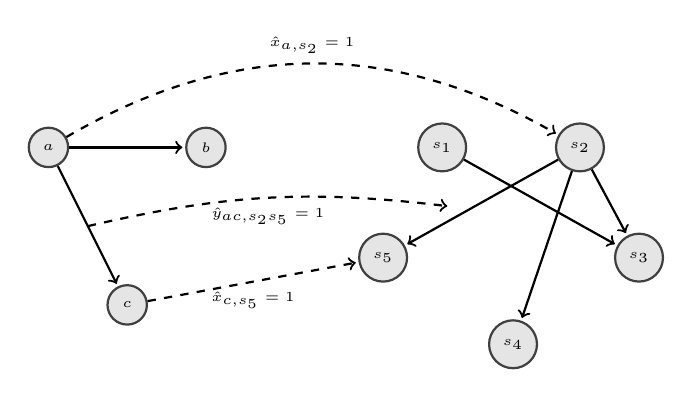
\begin{tikzpicture}[shorten >=1pt,->,scale=0.5]  
		        \tikzstyle{node}=[circle,thick,draw=black!75,fill=black!10,minimum size=5mm]
		        \tikzstyle{edge}=[draw, thick]
		    	\begin{scope}
			         \node [node] (a) at (0,4) {\tiny{$a$}};
			         \node [node] (b) at (4,4) {\tiny{$b$}};
			         \node [node] (c) at (2,0) {\tiny{$c$}};
			         \path[edge] (a) to  (b);
			         \path[edge] (a) to  (c);
			            
			         \node [node] (s1) at (10,4) {\tiny{$s_1$}};
			         \node [node] (s2) at (13.5,4) {\tiny{$s_2$}};
			         \node [node] (s3) at (15,1.2) {\tiny{$s_3$}};
			         \node [node] (s4) at (11.8,-1) {\tiny{$s_4$}};
			         \node [node] (s5) at (8.5,1.2) {\tiny{$s_5$}};

			         \path[edge] (s1) to (s3);
			         \path[edge] (s2) to (s3);
			         \path[edge] (s2) to (s4);
			         \path[edge] (s2) to (s5);
			         
			         \path[edge,dashed, bend left=30] (a) to  [above] node[font=\tiny] {$\hat{x}_{a,s_2}=1$} (s2);

			         \path[edge,dashed] (c) to  [below] node[font=\tiny] {$\hat{x}_{c,s_5}=1$} (s5);

			         \path[edge,dashed, bend left=10] (1,2) to  [below] node[font=\tiny] {$\hat{y}_{ac,s_2s_5}=1$} (10.2,2.5);
		         \end{scope}

		      \end{tikzpicture}
		      \\
		      ($p_u$) \hspace{2cm} ($g$)
		\end{tabular}
	\end{center}
   \caption{An illustration of matching variables for overlaying graph $g$ with coherence pattern $p_u$.}
   \label{fig:mapping-var}

\end{figure}

Given the above variables, we need to define some constraints in order to check if pattern $p_u$ is an induced subgraph of the selected nodes in projection graph $g$. 
To do so, we explain constraints which are used to check if a pattern is an induced subgraph of a projection graph or not. 

\begin{itemize}
\item Every node of the pattern matches at most one unique node of the graph:

\begin{equation}
\sum_{k\in V_g}\hat{x}_{i,k} \leq 1 \quad \forall i\in V_{p_{u}},
\end{equation}

\item Every edge of the pattern matches at most one unique edge of the graph:

\begin{equation}
\sum_{kl\in E_g}\hat{y}_{ij,kl} \leq 1 \quad \forall (i,j)\in E_{p_{u}},
\end{equation}

\item Every node of the graph matches at most one node of the pattern:

\begin{equation}
\sum_{i\in V_{p_{u}}}\hat{x}_{i,k} \leq 1 \quad \forall k\in V_g,
\end{equation}

\item A node of pattern $p_u$ matches a node of graph $g$ if an edge originating from the node of pattern $p_u$ matches an edge originating from the node of $g$:

\begin{equation}
\sum_{kl \in E_g}\hat{y}_{ij,kl} =  \hat{x}_{i,k}\textit{  }\forall k \in V_g, \textit{  }\forall ij \in E_{p_{u}},
\end{equation}

\item A node of pattern $p_u$ matches a node of graph $g$ if an edge targeting the node of pattern $p_u$ matches an edge targeting the node of $g$:

\begin{equation}
\sum_{kl \in E_g}\hat{y}_{ij,kl} =  \hat{x}_{j,l}\textit{  }\forall l \in V_g,\textit{  }\forall (i,j) \in E_{p_{u}},
\end{equation}

\item Following constraint ensures that the model extracts induced patterns.  
Pattern $p_{u}$ is an induced subgraph of graph $g$ if $p_{u}$ contains all possible edges that are present in $g$. 
So

\begin{equation}
\sum_{i \in V_{p_{u}}}\hat{x}_{i,k} + \sum_{j \in V_{p_{u}}}\hat{x}_{j,l} - \sum_{(i,j)\in E_{p_{u}}}\hat{y}_{ij,kl} \leq 1
 \quad\textit{  }\forall (k,l)\in E_g
\end{equation}
\end{itemize}

The above constraints check whether the pattern is an induced subgraph of the projection graph. 
But we must also check if the pattern occurs in a subgraph of the projection graph such that the subgraph contains only selected sentence nodes for producing the summary. 
In simple words, all associated sentences to the pattern nodes must be selected for the summary. 
So we define some more constraints in this regard:

\begin{itemize}

\item If sentences $s_{k}$ and $s_{l}$ are selected for the summary then the edge between them must be selected $(\hat{z}_{kl}=1)$ as well.
\begin{equation}
	\label{eq:quadretic-const}
 s_{k} \cdot \hat{s}_{l}=\hat{z}_{kl} \quad \forall k,l \in V_{g}
\end{equation}

\item Pattern $p_u$ is present in the summary ($\hat{p}_u=1$) if and only if one of its instances in the projection graph is included in the summary, i.e.,\ some of the selected sentence nodes must be present in an instance of pattern $p_{u}$.
Let $|V_{p_{u}}|$ be the number of nodes and $|E_{p_u}|$ be the number of edges in pattern $p_{u}$ then this constraint can be formulated as follows:

\begin{equation}
\underset{i \in V_{p_u}}{\sum} \underset{k \in V_g}{\sum} \hat{s}_k \cdot \hat{x}_{i,k}+\underset{ij \in e_{p_u}}{\sum} \underset{kl \in E_g}{\sum} \hat{z}_{kl} \cdot \hat{y}_{ij,kl} = \hat{p}_{u}(|V_{p_u}|+|E_{p_u}|)
\end{equation}

\item If a sentence node is selected then it must match a node of at least one of the patterns:

\begin{equation}
\sum_{p_{u} \in P} \sum_{i \in V_{p_{u}}} \hat{x}_{i,k} \geq \hat{s}_{k} \quad \forall k \in V_{g}
 \end{equation}
\end{itemize}

Now we can set up our experiments for evaluating our approach to coherence patterns on the summarization task. 

\subsubsection{Data}
We evaluate our model on two datasets:  \emph{PLOS medicine} and \emph{DUC 2002}. 
The PLOS medicine dataset consists of $50$ scientific articles.  
We are motivated to evaluate our model on scientific articles because of the growth in the number of scientific publications in different research fields.  
A summarizer assists researchers to have an informative and coherent gist of long scientific articles. 
Moreover, summarizing scientific articles is difficult as multi-document summarization because scientific articles tend to be long and important information is spread all over an article,  unlike the distribution of information in a news article \cite{teufel02}. 
The reason that we selected the PLOS medicine dataset is that articles in this dataset are accompanied by summaries written by editors of the month. 
Editors' summaries have a broader perspective than abstracts of articles.  
We use scientific articles and their corresponding editor's summaries as dataset $D$ in our formulation for the summarization task (see Section \ref{sec:auto-summarization}). 
Abstracts of scientific articles can be taken as summaries of articles as well. 
We collect abstracts of $700$ scientific articles from the PubMed\footnote{\url{http://www.ncbi.nlm.nih.gov/pmc/tools/ftp/}} corpus, which is in the \mbox{bio-medicine} field, to mine coherence patterns and compute their weights. 
This dataset of abstracts is dataset $H$ in our formulation for the summarization task.  
The articles of this dataset do not overlap with articles in PLOS Medicine dataset. 

We also evaluate our model on the DUC 2002 dataset that has been annotated for the Document Understanding Conference 2002. 
It contains $567$ news articles for summarization. 
Every article in this dataset is associated with at least two gold summaries written by humans. 
This is dataset $D$ in our formulation, and we use this dataset for the evaluation purposes. 
We use human summaries in the DUC 2005 dataset, which has $300$ articles, to mine coherence patterns and then calculate the weights of patterns.  
This is dataset $H$ in our formulation. 

DUC 2002 articles are shorter than \emph{PLOS Medicine}\ articles (25 vs.\ 154 sentences average\ length). 
In scientific papers clarity is paramount, so the author will endeavor to state things explicitly and avoid ambiguity. 
Authors of scientific articles repeat terminologies to be explicit.     
In contrast, in literature, word repetition is not only uncommon, but it is usually a sign of bad writing. 

\subsubsection{Experimental settings}
In the preprocessing phase, we extract texts from scientific articles by removing all figures, tables, references and \mbox{non-alphabetical} characters.
For both datasets, we use the Stanford parser \cite{klein03b} to parse sentences. 
We represent each text by its entity graph that is obtained based on its entity grid representation. 
We employ the Brown coherence toolkit \cite{elsner11b} to build entity grids from parse trees.  
We use gSpan \cite{yanxifeng02} to extract all coherence patterns from the projection graphs in $GS_H$. 
We use coherence patterns with three and four nodes to which we refer as 3-node and 4-node patterns respectively. 
The optimization is formulated as Mixed Integer Programming (MIP) that deals with quadratic constraints, like the constrain in Equation \ref{eq:quadretic-const}.  
We use Gurobi \cite{gurobi14} to solve the MIP optimization problem.
The values of weights of the importance, non-redundancy and coherence functions are set as 
$\lambda_{I}=0.4$, $\lambda_R=0.3$, and $\lambda_{c}=0.3$ for the \emph{PLOS Medicine}\ data set.  
Weights for the DUC 2002 development set are $\lambda_{I}=0.5$, $\lambda_R=0.2$ and $\lambda_{c}=0.3$.
Once a summary is produced, all pronouns in the summary are substituted with their antecedents using the pronoun resolution system provided by \newcite{martschat13}. 
We limit the length of summaries to $5$ sentences,  where we compare our system with the \mbox{state-of-the-art} systems on PLOS Medicine. 
However, since the word length limit of a summary is more reasonable than the sentence length limit of a summary, in addition we compare the examined summarization models where the length of a summary is restricted to the average length of editor's summaries in the dataset ($750$ words). 

\subsubsection{Compared summarization systems}
We compare our summarization system, which is enriched with coherence patterns, with the following summarization systems: 

\begin{itemize}
	\item \emph{Random}: This model selects sentences randomly from the input document;

	\item \emph{Lead}: This model takes the top n\% of the sentences of the input document\footnote{In our experiment it extracts five first sentences of articles};

	\item \emph{Maximal Marginal Relevance (MMR)} \cite{carbonell98}: This model uses a \mbox{trade-off} between relevance and redundancy to rank sentences. 
	 To do this, the model defines a linear ranking function as:
	 \begin{equation}
	 MMR(s_i) = \mathtt{\argmax}_{s_i}\lbrace \gamma sim(s_i,title) + (1-\gamma)\mathtt{\max}_{s_j}sim(s_i,s_j)) \rbrace 
	 \end{equation} 
	 where $\gamma$ is the trade-off factor. 
	 If $\gamma$ equals to one then the sentences in the input document are ranked merely based on their similarity with the title, which means ranking based on relevance. 
	 If $\gamma$ equals to zero, sentences are ranked based on the similarity among themselves, which can be interpreted as redundancy. 

    \item \emph{Text-Rank} \cite{mihalcea04b}: This graph-based model allows for the ranking of sentences that are recursively computed based on the information drawn from the entire text. 
    It represents the input document by a graph whose nodes represent sentences and edges indicate the existence of content overlaps between sentences. 
    Edges are weighted by the number of content words that overlap between sentences. 
    The ranking of sentences is measured by computing the importance of its corresponding node in the graph. 
    The node importance in the graph is computed based on the global information which is recursively drawn from the entire graph. 
    The importance score of each node in each recursion is updated concerning the importance score of its neighbors in the graph. 
    
    \item \emph{EntOD} \cite{parveen15a}: 
    This model uses ILP in order to optimize the summary based on importance, non-redundancy, and coherence. 
    The importance and \mbox{non-redundancy} components are identical to these components in the summarization system that is explained here. 
    The only difference between the EntOD system and our summarization system is in the coherence component. 
    In EntOD, the input document is represented by the entity graph to encode \mbox{entity-based} relations among sentences. 
    Then the outdegree of a node in the projection graph representation of the input document is taken as a measure of the contribution of each sentence to the coherence of the summary. 
    That is why we refer to this model as EntOD. 

    \item \emph{TopicOD} \cite{parveen15b}: 
    This summarization system is the same as the EntOD system except in the way that texts are represented. 
    TopicOD uses topical graphs, instead of entity graphs, to encode topical relations among sentences. 
    Topical graphs are bipartite graphs consisting of two sets of nodes: sentences and topics. 
    The outdegree of each sentence in weighted projection graphs is taken as the coherence measure of the sentence.

    \item \emph{Mead} \cite{radev04b}: This model assigns a score to each sentence of the input document using three scores. The centroid score, which is a measure of the centrality of a sentence to the overall topic of the input document; the position score, which decreases linearly as the sentence gets farther from the beginning of the input document; and the \mbox{overlap-with-first} score, which is the inner product of the TF*IDF-weighted vector representations of a sentence and the first sentence, or the title of the input document if it has one.  
    MEAD discards sentences that are too similar to other sentences (based on the cosine similarity). 
    Any sentence which is not discarded due to high similarity and which obtains a high score (within the specified compression rate) is included in the summary. 
	
\end{itemize}


\subsubsection{Results }
We evaluate the summarization system, which is enriched by coherence patterns in two ways. 
First, we use ROUGE scores to compare our summarizer with other models. 
Second, we explicitly evaluate the coherence of summaries by human judgments.

\paragraph{ROUGE assessment.}
The ROUGE score \cite{linchinyew04} is a standard evaluation metric for automatic text summarization. 
It principally measures word overlaps between gold summaries (usually generated by humans) and summaries produced by a model. 
ROUGE-1, ROUGE-2, and ROUGE-SU4 are three versions of ROUGE that are popularly reported for comparing different summarization systems. 
ROUGE-1 and ROUGE-2 capture unigram and bigram overlap between a gold summary and a produced summary. 
These are meant to assess informativeness. 
ROUGE-SU4 captures skip-bigram plus unigram-based co-occurrence statistics. 
We refer interested readers to  \newcite{graham15} for more explanations about evaluation metrics for the summarization task. 

Table \ref{table:plos_5len_editor} reports ROUGE scores of different systems on the \emph{PLOS Medicine} dataset where the length of the summaries is limited to five sentences. 
Our summarization system that uses three nodes outperforms other systems.  
It works better than EntOD and TopicOD systems showing that our coherence patterns are more informative than the average outdegree feature. 


\begin{table}[!ht]
	\begin{center}
		\begin{tabular}{lcc}
		\toprule
		\textbf{Systems} 			& \textbf{ROUGE-SU4} &\textbf{ROUGE-2}\\
		\midrule
		Lead 				& 0.067 	& 0.055  \\
		Random 				& 0.048  	& 0.031  \\
		MMR 				& 0.069 	& 0.048  \\
		TextRank 			& 0.068  	& 0.048  \\
		Mead 				& 0.084 	& 0.068  \\
		EntOD 				& 0.131		& 0.098  \\
		TopicOD				& 0.129 	& 0.095  \\
		\textbf{3-node} 				& \textbf{0.135} & \textbf{0.103} \\
		\bottomrule
		\end{tabular}
	\end{center}
	\caption{
	ROUGE scores on PLOS Medicine, editor's summaries with five sentences.}
	\label{table:plos_5len_editor}
\end{table}


Table \ref{tab:plos-750words} shows the performance of different systems with $750$ words limit for a summary where editor's summaries are taken as gold standard. 
We calculate different variations of ROUGE-2 and ROUGE-SU4. 
These variations demonstrate the effect of stop words and stemming in the ROUGE calculation.
For the sake of brevity, we use the notation ``SW'' to refer to stop words and ``SM'' to refer to word stemming.  
``SW--'' shows that stop words are not taken into account in ROUGE calculation; ``SW+'' is the opposite. 
``SM--'' shows that Porter Stemmer is not applied to summaries in ROUG calculation, ``SM+'' is its opposite. 
 
Our model achieves the best performance in comparison to other examined systems with respect to all variations of ROUGE. 
When we integrate coherence patterns with three nodes into the summarizer, i.e.\ 3-node, the summarizer significantly outperforms EntOD that uses the outdegree of sentence nodes as the coherence feature.   
These results confirm our argument at the beginning of this section: The outdegree of nodes in the projection graph of the input document is not a powerful representative for the coherence of selected sentences for a summary. 
3-node works better than EntOD basically because our coherence patterns capture the connectivity style among selected sentences from the input document for the summary, whereas
the outdegree measures to what extent a sentence is connected to other sentences in the input document, rather than the summary. 
Moreover, the outdegree does not capture how sentences should be connected to have a coherent summary.  

\begin{table}[!ht]
	\begin{center}
		\begin{tabular}{lr@{}lrrr||r@{}lrrr}
		\toprule
		\emph{PLOS Medicine}& \textbf{SW--}& & \textbf{SW--} & \textbf{SW+} & \textbf{SW+}& \textbf{SW--} & & \textbf{SW--} & \textbf{SW+} & \textbf{SW+} \\
		\textbf{Editor's summaries}  & \textbf{SM--} & & \textbf{SM--} &  \textbf{SM+} & \textbf{SM--} &  \textbf{SM+}  & & \textbf{SM--} &  \textbf{SM+}  & \textbf{SM--} \\
		\midrule
		&& \multicolumn{4}{c||}{ROUGE-SU4 ($\ast p<.05$)} & \multicolumn{4}{c}{ROUGE-2 ($\ast p<.01$)}\\
		\midrule
		Random &  0.140& & 0.113 & 0.169  & 0.153 &  0.102 & & 0.088 & 0.125 & 0.116 \\
		Lead & 0.191 & & 0.158 & 0.246 & 0.222  & 0.158 & & 0.140 &0.185 &0.171   \\
		MMR & 0.183& & 0.149 & 0.240 & 0.215 & 0.141 & & 0.125 & 0.171 &0.157 \\
		TextRank & 0.148& & 0.104 & 0.161 & 0.159 & 0.115 & & 0.084 &0.126 & 0.118\\
		Mead & 0.197 & & 0.165 & 0.246 & 0.222& 0.156 & &0.139 & 0.186 & 0.172 \\
		EntOD & 0.204&* & 0.167 & 0.254& 0.228 &0.160 &* & 0.145 &0.187 & 0.173\\
		TopicOD & 0.195 & &0.161 & 0.231 &0.206 & 0.157 &  & 0.140 &0.169 & 0.165 \\
		3-node &0.215& * &0.178& 0.268& 0.241& 0.172 & * & 0.153 & 0.200 &0.184 \\
		\textbf{4-node} & \textbf{0.218}& & \textbf{0.179} & \textbf{0.270} & \textbf{0.245}  & \textbf{0.175} & & \textbf{0.156} & \textbf{0.201} & \textbf{0.187} \\
		\bottomrule
		\end{tabular}
	\end{center}
	\caption{ROUGE scores on PLOS Medicine with 750 words.}
	\label{tab:plos-750words}
\end{table}
	
When we integrate 4-node coherence patterns into the summarizer, the summarizer works slightly better than when 3-node patterns are combined. 
This confirms that large subgraphs capture more information about the connectivity style of nodes in a projection graph and therefore the coherence of sentences.  
However, this improvement is not statistically significant. 
4-node patterns are less likely than 3-node patterns to occur in a subgraph of the projection graph where the subgraph contains only selected nodes for the summary. 

The summarizer that is enriched by our coherence patterns outperforms \emph{Mead} as one of the strong summarization systems. 
Summaries produced by \emph{Mead} on average contain fewer sentences than summaries produced by 3-node patterns (17.5 vs. 27.2 sentences per summary).
This shows that \emph{Mead} selects longer sentences in comparison to our 3-node patterns.  
Long sentences are more complicated, less readable, and may also contain more irrelevant entities than short sentences. 

Table \ref{tab:summary-duc} shows the results on DUC 2002 of well-performed systems in the previous experiment. 
In addition to other models, we compare our model to \emph{NN-SE} that utilizes a neural network hierarchical document encoder and an \mbox{attention-based} extractor to extract sentences from a document for a summary \cite{chengjianpeng16}.

ROUGE scores of our summarization approach, i.e.\ 3-node in Table \ref{tab:summary-duc}, on this dataset surpass the scores of other summarization systems. 
This shows that our system performs well even in a different domain and with considerably shorter input documents. 
Our model outperforms the \emph{NN-SE} system because our model explicitly takes into account the connectivity of selected sentences in the sentence extraction phase. 
We only use 3-node subgraphs on this dataset because the summaries are supposed to be very short. 
So 3-node subgraphs are sufficient to capture the connectivity style of selected sentences. 


\begin{table}[!ht]
	\begin{center}
		\begin{tabular}{lccc}
			\toprule
			\textbf{Systems} 					& \textbf{ROUGE-1} 	& \textbf{ROUGE-2} 	& \textbf{ROUGE-SU4} \\
			\midrule
			Lead 						& 0.459 & 0.180 & 0.201	\\
			TextRank 					& 0.470 & 0.195 & 0.217	\\
			DUC 2002 Best 				& 0.480 & 0.228 & 		\\
			Mead 						& 0.445 & 0.200 & 0.210	\\
			EntOD						& 0.485 & 0.230 & 0.253 \\
			TopicOD 					& 0.481 & 0.243 & 0.242 \\
			NN-SE 						& 0.474 & 0.230 & 		\\
			\textbf{3-node} 						& \textbf{0.490} & \textbf{0.247} & \textbf{0.258}\\
			\bottomrule
		\end{tabular}
	\end{center}
	\caption{ROUGE scores on DUC 2002.}
	\label{tab:summary-duc}
\end{table}

\paragraph{Coherence Assessment.} 
Here we exclusively assess the coherence aspect of summaries by asking human judges to rank summaries that are generated by different systems. 
To this end, we ask four human judges\footnote{Human judges are one PostDoc, two Ph.D. students and one Masters student in our NLP group.} to rank summaries of four different systems for ten different articles. 
The most coherent summary is assigned with rank $1$, the second best is assigned with rank $2$, the third best gets rank $3$, and the worst obtains rank $4$.
The four summarization systems are
\emph{3-node}, \emph{EntOD}, \emph{Text-Rank}, and \emph{Lead}.

The Kendall concordance coefficient (W) \cite{siegel88} over the rankings is calculated in order to measure the agreement between the human judges.  
We calculate Kendall's W for every scientific article, which is given to the human subjects. 
Then, we calculate the average of Kendall's W of scientific articles. 
The average Kendall's W is $0.6725$, which indicates a high level of agreement between human subjects.
Applying the $\chi^2$ statistical test shows that W is statistically significant (p\_value <.05) indicating that the rankings provided by the human judges are reliable and informative.


\begin{table}[!ht]
	\begin{center}
		\begin{tabular}{lc}
		\toprule
		\textbf{System} 				&  \textbf{Average human scores} \\
		\midrule
		TextRank 			& 3.950					\\
		EntOD 				& 2.325					\\
		\textbf{3-node}		& \textbf{1.875} 		\\
		Lead 				& 1.625					\\
		\bottomrule
		\end{tabular}
	\end{center}
	\caption{The average human scores evaluated on the PLOS Medicine dataset. Lower is better. 
	The bold line is our system.}
	\label{tab:summary-human}
\end{table}

Table \ref{tab:summary-human} shows the overall average rankings summaries produced by a system received by human judges. 
\emph{Lead} obtains the best overall average rank because it extracts adjacent sentences from the beginning of the text. 
Hence, the summaries produced by this system are coherent as the author intends them to be. 
Our summarizer, which is enriched with 3-node coherence patterns, follows LEAD by outperforming EntOD and TextRank, showing that the integration of our coherence patterns into the summarization system yields texts that are more coherent in comparison to summaries that are produced by baseline summarizers such as EntOD that uses the average outdegree.  

\section{Summary}
\label{sec:summary}

In this chapter, we challenged the average outdegree metric that is heuristically defined by the entity graph model. 
The primary intuition behind the usage of this metric is that documents whose projection graphs have higher average outdegrees than others are more coherent. 
We showed that the average outdegree of nodes in a projection graph is not sufficient to capture the connectivity style of nodes and consequently the perceived coherence of the corresponding document. 
Instead, we proposed novel coherence patterns that capture the entity-based connectivity style of sentences in documents. 
We employed projection graphs of texts in a corpus to encode the connectivity style of sentences.  
Then by applying a subgraph mining algorithm to all projection graphs of all texts, we mine all occurring subgraphs in these graphs as coherence patterns. 
We use the frequency of each coherence pattern in a projection graph as a  feature of the connectivity style of nodes in the projection graph and consequently, a feature of the perceived coherence of the corresponding document. 

We evaluated our coherence patterns in two applications: readability assessment and extractive \mbox{single-document} summarization. 
In the former, we observed that frequencies of some coherence patterns positively and some others negatively correlate with readability ratings, which are assigned to texts by human judges. 
Positively correlated patterns mostly depict the intuition in texts that a sentence introduces some entities, and its subsequent sentences elaborate on each of them.  
Negatively correlated patterns roughly remind us of the linear chain pattern in linguistics where a sentence is located between two sentences with different topics to make the topic change smooth across sentences. 
This pattern is an indicator of a topic shift.  
Although topic shifts make a text appealing, too frequent occurrences of this pattern in a document disturb the readability of the document. 
Our experiments showed that 4-node subgraphs are more predictive than 3-node subgraphs in ranking documents with respect to their readability. 
We believe that this is mainly because large coherence patterns have more capacity than small ones for encoding the connectivity style of nodes in projection graphs. 

In the summarization task, we examined our coherence patterns by integrating them into an existing summarization system that is developed on the entity graph representation of documents. 
This task was challenging because we had to model the existence of our coherence patterns in summary by defining several new constraints in linear programming.  
The results of our experiments on DUC 2002 as a standard dataset for summarization and PLOS Medicine as a corpus of scientific articles show that our coherence patterns improve the performance of the summarizer with respect to ROUGE and human evaluation. 


The key message of this chapter is that in order to capture the connectivity style of sentences in a document, which is encoded via the graph representation of the document, coherence patterns, which are obtained automatically by applying a subgraph mining algorithm to graphs, are more useful than average outdegree, which is designed heuristically. 
Coherence patterns capture coherence by taking each sentence in its connections with other sentences in the text. 
Our \mbox{data-driven} approach to coherence pattern mining enables our model to extract patterns from documents so that a machine learning model can learn relations among the patterns systematically. 

We observe that 4-node subgraphs are better coherence patterns than 3-node subgraphs. 
However, more investigation is required to be performed on how the size of subgraphs influences the performance of the model. 
The entity graph does not include mentions that are semantically related.  
It is restricted to only noun overlap relation among nouns in sentences, while any lexical semantic relation between words in sentences can relate sentences. 
We follow these points in the following chapter of this thesis. 

The main contributions of the research in this chapter are:

\begin{itemize}
\item assessing the average outdegree metric for coherence measurement,
\item proposing subgraphs of projection graphs as coherence patterns and their frequencies as features which encode coherence, 
\item evaluating our coherence patterns in ranking texts with respect to their coherence property,
\item showing how coherence patterns can be utilized in readability assessment as a text quality evaluation task, and the document summarization task as an instance of text generation systems.   
\end{itemize}


